%definira klasu dokumenta 
\documentclass[12pt]{report} 

%prostor izmedu naredbi \documentclass i \begin{document} se zove uvod. U njemu se nalaze naredbe koje se odnose na cijeli dokument

%osnovni LaTex ne može riješiti sve probleme, pa se koriste različiti paketi koji olakšavaju izradu željenog dokumenta
\usepackage[croatian]{babel} 
\usepackage{amssymb}
\usepackage{amsmath}
\usepackage{txfonts}
\usepackage{mathdots}
\usepackage{titlesec}
\usepackage{array}
\usepackage{lastpage}
\usepackage{etoolbox}
\usepackage{tabularray}
\usepackage{color, colortbl}
\usepackage{adjustbox}
\usepackage{geometry}
\usepackage[classicReIm]{kpfonts}
\usepackage{hyperref}
\usepackage{fancyhdr}

\usepackage{float}
\usepackage{setspace}
\restylefloat{table}

%added
\usepackage{wrapfig}
\usepackage{caption}
\captionsetup{font=small}
%


\patchcmd{\chapter}{\thispagestyle{plain}}{\thispagestyle{fancy}}{}{} %redefiniranje stila stranice u paketu fancyhdr

%oblik naslova poglavlja
\titleformat{\chapter}{\normalfont\huge\bfseries}{\thechapter.}{20pt}{\Huge}
\titlespacing{\chapter}{0pt}{0pt}{40pt}


\linespread{1.3} %razmak između redaka

\geometry{a4paper, left=1in, top=1in,}  %oblik stranice

\hypersetup{ colorlinks, citecolor=black, filecolor=black, linkcolor=black,	urlcolor=black }   %izgled poveznice


%prored smanjen između redaka u nabrajanjima i popisima
\newenvironment{packed_enum}{
	\begin{enumerate}
		\setlength{\itemsep}{0pt}
		\setlength{\parskip}{0pt}
		\setlength{\parsep}{0pt}
	}{\end{enumerate}}

\newenvironment{packed_item}{
	\begin{itemize}
		\setlength{\itemsep}{0pt}
		\setlength{\parskip}{0pt}
		\setlength{\parsep}{0pt}
	}{\end{itemize}}




%boja za privatni i udaljeni kljuc u tablicama
\definecolor{LightBlue}{rgb}{0.9,0.9,1}
\definecolor{LightGreen}{rgb}{0.9,1,0.9}

%Promjena teksta za dugačke tablice
\DefTblrTemplate{contfoot-text}{normal}{Nastavljeno na idućoj stranici}
\SetTblrTemplate{contfoot-text}{normal}
\DefTblrTemplate{conthead-text}{normal}{(Nastavljeno)}
\SetTblrTemplate{conthead-text}{normal}
\DefTblrTemplate{middlehead,lasthead}{normal}{Nastavljeno od prethodne stranice}
\SetTblrTemplate{middlehead,lasthead}{normal}

%podesavanje zaglavlja i podnožja

\pagestyle{fancy}
\lhead{Programsko inženjerstvo}
\rhead{DentAll}
\lfoot{Potplaćeni}
\cfoot{stranica \thepage/\pageref{LastPage}}
\rfoot{\today}
\renewcommand{\headrulewidth}{0.2pt}
\renewcommand{\footrulewidth}{0.2pt}

\begin{document} 
	
	
	
	\begin{titlepage}
		\begin{center}
			\vspace*{\stretch{1.0}} %u kombinaciji s ostalim \vspace naredbama definira razmak između redaka teksta
			\LARGE Programsko inženjerstvo\\
			\large Ak. god. 2023./2024.\\
			
			\vspace*{\stretch{3.0}}
			
			\huge DentAll\\
			\Large Dokumentacija, Rev. 0.1\\
			
			\vspace*{\stretch{12.0}}
			\normalsize
			Grupa: Potplaćeni\\
			Voditelj: Luka Kokić\\
			
			
			\vspace*{\stretch{1.0}}
			Datum predaje: \textit{17.11.2023.}\\
	
			\vspace*{\stretch{4.0}}
			
			Nastavnik: \textit{Goran Rajić}\\
		
		\end{center}

	
	\end{titlepage}

	
	\tableofcontents


	\chapter{Dnevnik promjena dokumentacije}
				
		\begin{longtblr}[
				label=none
			]{
				width = \textwidth, 
				colspec={|X[2]|X[10]|X[6]|X[3]|}, 
				rowhead = 1
			}
			\hline
			\textbf{Rev.}	& \textbf{Opis promjene/dodatka} & \textbf{Autori} & \textbf{Datum}\\[3pt] \hline
			0.1 & Napravljen predložak	& Luka Kokić & 25.10.2023. 		\\[3pt] \hline 
			0.2 & Opis projektnog zadatka + (partial) Specifikacija programske potpore	& Ian Marković & 31.10.2023. 		\\[3pt] \hline 
			0.3 & Dodani opis arhitekture baze podataka kao i relacijska shema	& Karlo Baljak & 31.10.2023. 		\\[3pt] \hline 
			0.4 & Početna verzija obrazaca uporabe & Ian Marković, Teo Musa & 9.11.2023. 		\\[3pt] \hline 
			0.5 & Konačna verzija obrazaca uporabe i ostali zahtjevi & Ian Marković, Teo Musa & 10.11.2023. 		\\[3pt] \hline 
			0.6 & Početak dijagrama obrazaca uporabe & Mislav Matić & 11.11.2023. 		\\[3pt] \hline 
			0.7 & Dijagrami razreda & Karlo Baljak & 11.11.2023. 		\\[3pt] \hline 
			0.8 & Dovršeni dijagrami obrazaca uporabe & Mislav Matić, Luka Kokić & 15.11.2023. 		\\[3pt] \hline 
			0.9 & Početak sekvencijskih dijagrama & Bruno Milaković & 15.11.2023. 		\\[3pt] \hline 
			0.10 & Dovršeni sekvencijski dijagrami & Bruno Milaković, Luka Kokić & 16.11.2023. 		\\[3pt] \hline
			
			

		\end{longtblr}
	\chapter{Opis projektnog zadatka}
		%nas sadrzaj
		Cilj ovog projekta je razviti web aplikaciju „DentAll“ kojom će pružatelji usluga zdravstvenog turizma moći evidentirati i koordinirati lokalni smještaj i prijevoz korisnika usluga. Time bi se zdravstveni turizam učinio privlačnijim rješavanjem brige i cijene smještaja i prijevoza korisnika pri njihovom obitavanju u mjestu gdje koriste spomenute usluge. Uz to bi klijenti pružatelja usluga bili u mogućnosti unaprijed vidjeti geografsku sliku smještaja i okolice te moguće turističke opcije i kretanja tijekom privremenog obitavanja .
		
		\smallskip
		Aplikacija bi olakšala brige vlasnika usluga zdravstvenog turizma evidentiranjem, organizacijom i praćenjem smještaja i prijevoza klijenata uz programsku podršku interneta. Time se nastoji nadomjestiti nedostatak ovisnosti pružatelja zdravstvenih usluga o raznim i višestrukim pružateljima smještajnih usluga. Takvim pristupom kroz javnu i lagano dostupnu uslugu smanjio bi se broj posrednika u organizaciji i administraciji pružanja usluga zdravstvenog turizma. Također bi klijenti pronalazili sve potrebne informacije oko odabranog zdravstvenog turizma, tj. uz same zdravstvene usluge i o smještaju te prijevozu za svaki termin, čineći sam odabir prisustvovanja u inozemnim zdravstvenim uslugama jednostavniji i privlačniji.
		
		\smallskip
		Trenutna postojeća rješenja uključuju korištenje hotela i motela, što čini cijeli proces zdravstvenog turizma skupljim i kompliciranijim. Dugoročno bi pružateljima bilo isplativije iznajmljivati vlastite nekretnine u sklopu pružanja cjelokupnih usluga. Također je u trenutnim rješenjima prijevoz ostavljen na odgovornost klijenata, što otežava korištenje cijele usluge i njezinu privlačnost. Spajanjem oba problema u jedan sustav bi učinilo uslugu zdravstvenog turizma puno efektivnijom i jeftinijom, a time i više privlačnom mogućim budućim klijentima.
		
		\smallskip
		\noindent Postojeće vrste konkurentnih rješenja:
		\begin{packed_item}
			\item  javno dostupne informacije o načinima sudjelovanja u zdravstvenom turizmu i pripadnim članovima
			\item  udruge sa svrhom spajanja svih dionika pružanja usluga zdravstvenog turizma
		\end{packed_item}
		
		\break
		\begin{wrapfigure}{r}{6cm}
			
\includegraphics[width=6cm]{slike/konkurencija.png} %veličina slike u odnosu na originalnu datoteku i pozicija slike
			\caption{Mogućnosti povezivanja klijenata i pružatelja koje nudi web stranica "MedicalTourism.com"}
			\label{fig:konkurencija}
			\centering
		\end{wrapfigure}
		
		Primjer za usluge pružanja informacija je web stranica „MedicalTourism.com“ koja pruža korisnicima podatke o pružateljima zdravstvenih usluga, smještaja i mogućih tretmana koje spomenute usluge pružaju. Također sadrži i mnoge druge informacije kao vodiče za destinacije, usporedbe cijena i slično. No ipak je spomenuta web aplikacija napravljena za pružanje laganog pristupa svim potrebnim informacijama za moguće klijente, pružatelje zdravstvenih usluga, pružatelje smještaja te osiguravajuća društva na jednom mjestu te se time ne sukobljava do konkurentske razine sa svrhom kreiranja projektne aplikacije.
		
		
		Dok je primjer druge vrste rješenja, čak konkurentnije ideji projekta, udruga Medical Tourism Association, koja spaja sve potrebne članove zdravstvenog turizma kroz program članstva. Udruga operira po cijelom svijetu i služi svrhu omogućavanja pružanja usluga zdravstvenog turizma kroz povezivanje potrebnih članova te svrhu informiranja javnosti o mogućnostima korištenja tih usluga. Također podržava edukaciju budućih pružatelja sa sveukupnim ciljem povećanja učestalosti zdravstvenog turizma u svijetu. Ovdje opisan projekt ipak sadrži određene funkcionalnosti koje nedostaju navedenoj konkurenciji, kao automatiziran proces organizacije i administracije, te lagano dostupni pregled informacija o obitavanju za klijente zdravstvenih usluga.
		
		
		%\begin{figure}[H]
		%	
\includegraphics[scale=0.4]{slike/konkurencija.png} %veličina slike u odnosu na originalnu datoteku i pozicija slike
		%	\raggedleft
		%	\caption{Prikaz procesa i mogućnosti usluga povezivanja klijenata i pružatelja usluga koju nudi web stranica "MedicalTourism.com"}
		%	\label{fig:konkurencija}
		%\end{figure}
		
		
		\break
		Ciljani klijenti opisanih usluga su pružatelji usluga zdravstvenog turizma po cijelom svijetu, uključujući Hrvatsku i slične države sa jeftinom cijenom boravka. Optimalno bi bilo započeti pružanje usluga aplikacije najprije Europskim državama i okolici, a zatim, uz dovoljnu uspješnost i isplativost projekta, raširiti dostupnost usluge ostatku svijeta. Ciljani klijenti bi također bili i pružatelji lokalnih prijevoznih usluga, od privatnih firmi do javnih taksija, koje bi aplikacija spajala sa pružateljima zdravstvenih usluga za dogovor o prijevozu njihovih klijenata. Također bi, u manjoj perspektivi, evidencija većine korisnika zdravstvenog turizma na jednom mjestu olakšala statističke analize razvoja zdravstvenog turizma po cijelom svijetu.
		
		\medskip
		U aplikaciji postoje tri uloge:
		\begin{packed_item}
			\item  smještajni administrator
			\item  administrator prijevoznih usluga
			\item  korisnički administrator
		\end{packed_item}
		
		Jedan korisnik može imati više administratorskih uloga, dok uloga smještajnog administratora sadrži najveće ovlasti kojima mogu definirati druge korisnike i dodjeljivati uloge. Svaka uloga administratora sadrži određene posebne mogućnosti dodavanja i promjene informacija.
		
		\smallskip
		Smještajni administratori upravljaju podatcima o smještaju; unose podatke o raspoloživom smještaju te definiraju smještajne kapacitete i unose ili brišu osnovne podatke o smještaju. Podatci smještaja se sastoje od tipa stana, kategorije opremljenosti, adrese i vremenskog perioda dostupnosti za korištenje. Uz svaki smještaj je dostupan grafički prikaz geografskog položaja uz Google Maps usluge.
		
		Administratori prijevoznih usluga upravljaju podatcima o prijevoznicima. To uključuje osnovne osobne i kontaktne podatke prijevoznika, vrstu i kapacitet prijevoznog sredstva te radno vrijeme raspoloživosti. Osnovni podatci prijevoznika se ne mogu mijenjati.
		
		Korisnički administratori definiraju korisnike medicinskih usluga uz unos njihovih osnovnih podataka. Podatci korisnika se sastoje od imena, prezimena, kontaktnih podataka, vremena dolaska i odlaska u/iz zemlje te preferencije o veličini i kvaliteti smještaja. Detalji njihovih tretmana se preuzimaju iz vanjske aplikacije o evidenciji medicinskih usluga.

		\break
		Aplikacija periodički provjerava status unesenih podataka i pridjeljuje adekvatni smještaj upisanim korisnicima te po zaključenju plana medicinskih usluga određenog korisnika im pridjeljuje prijevoznike od raspoloživih za svaki od termina. Sa završetkom spomenutog zaključenja sustav šalje poruku elektroničke pošte korisniku medicinskih usluga sa svim potrebnim informacijama te također šalje poruke elektroničke pošte prijevoznicima pridijeljenima terminima korisnika sa svim njima potrebnim informacijama.
		
		\medskip
		Moguće dodatne funkcionalnosti za aplikaciju koje se mogu nadodati nakon izvršavanja jezgrenih funkcionalnosti su:
		\begin{packed_item}
			\item  prijavljivanje samog korisnika medicinskih usluga u aplikaciju čime mogu provjeriti osobne podatke, smještaj, prijevoznike i termine
			\item  proširenje aplikacije u dodatnu svrhu prikaza općenitih podataka o medicinskom turizmu za privlačenje dodatnih klijenata
			\item  mogućnost pridjeljivanja istog smještaja većem broju pacijenata u slučaju da je smještaj dovoljno velik.
		\end{packed_item}
		\break
		%
	\chapter{Specifikacija programske potpore}
		
	\section{Funkcionalni zahtjevi}
			\noindent \textbf{Dionici:}
			\begin{packed_enum}
				\item Pružatelji zdravstvenih usluga (klinike)
				\item Pružatelji prijevoznih usluga (prijevoznici)
				\item Klijenti zdravstvenog turizma
				\item Korisnici (administratori)
				\begin{packed_enum}
					\item[a)] administratori smještaja
					\item[b)] administratori prijevoza
					\item[c)] korisnički administratori
				\end{packed_enum}
				\item Razvojni tim
				
			\end{packed_enum}
			
			\noindent \textbf{Aktori i njihovi funkcionalni zahtjevi:}
			
			
			\begin{packed_enum}
				\item  \underbar{Neregistrirani/neprijavljeni korisnik (inicijator) može:}
				\begin{packed_enum}
					\item pregledati informacije o dostupnim tretmanima i klinikama u odabranoj državi i gradu, te vidjeti raspoloživost tih usluga
					\item odabrati dostupan tretman i poslati zahtjev za primanje tretmana
					\item se prijaviti na postojeći korisnički račun upisivanjem korisničkog imena i lozinke
					\begin{packed_enum}
						
						\item  podfunkcionalnost 1 
						\item  podfunkcionalnost 2
				
					\end{packed_enum}
				\end{packed_enum}
			
				\item  \underbar{Administrator smještaja (inicijator) može:}
				\begin{packed_enum}
					\item unijeti, modificirati i brisati podatke o smještaju
					\item vidjeti postojeće smještaje, njihove podatke i raspoloživost (uz grafički prikaz)
					\item unijeti i brisati podatke o prijavljenim pružateljima medicinskih usluga
					\item vidjeti postojeće prijavljene pružatelje medicinskih usluga
					\item vidjeti postojeće korisnike
					\item registrirati nove korisnike te dodjeljivati uloge i brisati postojeće
				\end{packed_enum}
				
				\item  \underbar{Administrator prijevoznih usluga (inicijator) može:}
				\begin{packed_enum}
					\item unijeti i brisati podatke o prijevoznicima
					\item modificirati podatke raspoloživosti prijevoznika
					\item vidjeti postojeće podatke prijevoznika i njihove raspoloživosti
				\end{packed_enum}
				
				\item  \underbar{Korisnički administrator (inicijator) može:}
				\begin{packed_enum}
					\item unijeti i brisati podatke korisnika medicinskih usluga
					\item vidjeti postojeće korisnike medicinskih usluga i njihove podatke
					\item preuzeti i vidjeti detalje tretmana klinika u kontekstu korisnika medicinskih usluga
				\end{packed_enum}
				
					\item  \underbar{Baza podataka (sudionik):}
				\begin{packed_enum}
					\item pohranjuje sve podatke o korisnicima i njihovim ovlastima
					\item pohranjuje sve podatke o smještajima, raspoloživosti i smještajnim kapacitetima
					\item pohranjuje sve podatke o prijevoznicima
					\item pohranjuje sve podatke o korisnicima medicinskih usluga
					\item pohranjuje sve podatke o dogovorenim terminima boravka pacijenta i prijevoza tijekom boravka
				\end{packed_enum}
			\end{packed_enum}
			\eject 
			
			
				
			\subsection{Obrasci uporabe}
				
				\textbf{\textit{dio 1. revizije}}
				
				\subsubsection{Opis obrazaca uporabe}
					\textit{Funkcionalne zahtjeve razraditi u obliku obrazaca uporabe. Svaki obrazac je potrebno razraditi prema donjem predlošku. Ukoliko u nekom koraku može doći do odstupanja, potrebno je to odstupanje opisati i po mogućnosti ponuditi rješenje kojim bi se tijek obrasca vratio na osnovni tijek.}\\
					

					\noindent \underbar{\textbf{UC$<$broj obrasca$>$ -$<$ime obrasca$>$}}
					\begin{packed_item}
	
						\item \textbf{Glavni sudionik: }$<$sudionik$>$
						\item  \textbf{Cilj:} $<$cilj$>$
						\item  \textbf{Sudionici:} $<$sudionici$>$
						\item  \textbf{Preduvjet:} $<$preduvjet$>$
						\item  \textbf{Opis osnovnog tijeka:}
						
						\item[] \begin{packed_enum}
	
							\item $<$opis korak jedan$>$
							\item $<$opis korak dva$>$
							\item $<$opis korak tri$>$
							\item $<$opis korak četiri$>$
							\item $<$opis korak pet$>$
						\end{packed_enum}
						
						\item  \textbf{Opis mogućih odstupanja:}
						
						\item[] \begin{packed_item}
	
							\item[2.a] $<$opis mogućeg scenarija odstupanja u koraku 2$>$
							\item[] \begin{packed_enum}
								
								\item $<$opis rješenja mogućeg scenarija korak 1$>$
								\item $<$opis rješenja mogućeg scenarija korak 2$>$
								
							\end{packed_enum}
							\item[2.b] $<$opis mogućeg scenarija odstupanja u koraku 2$>$
							\item[3.a] $<$opis mogućeg scenarija odstupanja  u koraku 3$>$
							
						\end{packed_item}
					\end{packed_item}
				
					
				\subsubsection{Dijagrami obrazaca uporabe}
					
					\textit{Prikazati odnos aktora i obrazaca uporabe odgovarajućim UML dijagramom. Nije nužno nacrtati sve na jednom dijagramu. Modelirati po razinama apstrakcije i skupovima srodnih funkcionalnosti.}
				\eject		
				
			\subsection{Sekvencijski dijagrami}
				
				\textbf{\textit{dio 1. revizije}}\\
				
				\textit{Nacrtati sekvencijske dijagrame koji modeliraju najvažnije dijelove sustava (max. 4 dijagrama). Ukoliko postoji nedoumica oko odabira, razjasniti s asistentom. Uz svaki dijagram napisati detaljni opis dijagrama.}
				\eject
	
		\section{Ostali zahtjevi}
		
			\textbf{\textit{dio 1. revizije}}\\
		 
			 \textit{Nefunkcionalni zahtjevi i zahtjevi domene primjene dopunjuju funkcionalne zahtjeve. Oni opisuju \textbf{kako se sustav treba ponašati} i koja \textbf{ograničenja} treba poštivati (performanse, korisničko iskustvo, pouzdanost, standardi kvalitete, sigurnost...). Primjeri takvih zahtjeva u Vašem projektu mogu biti: podržani jezici korisničkog sučelja, vrijeme odziva, najveći mogući podržani broj korisnika, podržane web/mobilne platforme, razina zaštite (protokoli komunikacije, kriptiranje...)... Svaki takav zahtjev potrebno je navesti u jednoj ili dvije rečenice.}
			 
			 
			 
	
	\chapter{Arhitektura i dizajn sustava}
		
		Arhitektura sustava može se podijelit na tri glavna podsustava: web preglednik, web poslužitelj i baza podataka.
	\begin{itemize}
		\item 	\textbf{Web preglednik} – program koji služi za pristupanje web stranicama. Putem web preglednika korisnik komunicira sa poslužiteljem koristeći princip zahtjev-odgovor ili šalje podatke (najčešće u obliku obrazaca). Daljnja zadaća web preglednika je osigurati da se traženi podaci ispravno prikazuju ili da se ispravno prosljeđuju i spremaju na poslužitelj.
		\item 	\textbf{Web poslužitelj} – glavni je dio web aplikacije. To je most koji povezuje korisnika i bazu podataka koji se temelji na protokolu HTTP. Na zahtjeve korisnika dohvaća tražene podatke (resurse) ili obrađuje i sprema poslane podatke od korisnika.
		\item 	\textbf{Baza podataka} – srce je sustava. U njoj su pospremljeni svi podaci. Skoro ne postoji sustav u kojem nema komunikacije između aplikacije i baze.	
	\end{itemize}
		Aplikacije je izgrađena na modelu MVC (Model – View - Controller) softverske arhitekture uz male modifikacije. Controller dio strukture je ostvaren tako što je integriran unutar same baze, tj. funkcije koje manipuliraju podacima se nalaze unutar baze. Shodno tome aplikaciju onda dijelimo na tri komponente:
	\begin{itemize}
		\item	\textbf{Model} – glavna komponenta sustava. Reprezentira strukturu podataka.
		\item	\textbf{View} – komponenta zaslužna za reprezentaciju podataka.
		\item	\textbf{Controller} – komponenta koja odrađuje svu logiku i komunikaciju između sučelja i baze.
	\end{itemize}
	
		\smallskip
		Backend naše aplikacije je ostvaren direktno u bazi postgreSQL(razvojno sučelje pgadmin) za što koristimo API napisan u Node.js frameworku Express, koji služi kao middleware. Za izradu frontend-a korišten je React uz pomoć Material UI. Razvojno okruženje koje smo koristili je bilo Visual Studio Code.
		

		

				
		\section{Baza podataka}
			
			%\textbf{\textit{dio 1. revizije}}\\
			
		%\textit{Potrebno je opisati koju vrstu i implementaciju baze podataka ste odabrali, glavne komponente od kojih se sastoji i slično.}
			U ovom projektu koristit ćemo relacijsku bazu podataka, čije su osnovne jedinke entiteti, definirani imenom i skupom atributa. Osnovna zadaća baze podataka je pohrana podataka te brza i efikasna obrada tih podataka u ovisnosti i korisničkim zahtjevima. U bazi podataka su pohranjeni podaci o korisnicima, njihovim ulogama, preferencijama, kao i o smještaju te dostupnosti smještaja. Dodatno uz navedeno, zbog zahtjeva organizacije prijevoza, baza također sprema informacije o vrstama vozila i dostupnosti tih vozila kao i o vremenu i mjestu boravka korisnika zdravstvenog turizma. Tako su i definirani sljedeći entiteti:
			\begin{multicols}{2}
				\begin{itemize}
					\item Accommodation
					\item AccommodationOccupied
					\item AccommodationType
					\item AdminUser
					\item Assigned
					\item AssignedRole
					\item Clinic
					\item Credentials
					\item Equipped
					\item Patient
					\item PatientArrival
					\item PatientPlan
					\item PatientPreferences
					\item Town
					\item Transporter
					\item Treatment
					\item UserRole
					\item Vehicle
					\item VehicleOccupied
					\item VehicleSchedule
					\item VehicleType
				\end{itemize}
			\end{multicols}
		
			\subsection{Opis tablica}
			
				%Accommodation
				\textbf{Accommodation} Ovaj entitet sadrži podatke o smještaju, vrsti smještaja, njegovoj opremljenosti te adresi na kojoj se nalazi kao i koordinatama. Atributi su: AccommodationID (primary key), realEstateID, TypeID (foreign key), EquippedID (foreing key), latitude, longitude, address, TownID (foreign key), ClinicID (foreign key), active. Ovaj je entitet u vezi Many-to-One sa entitetom Town preko atributa TownID,u vezi Many-to-One sa entitetom Clinic preko atributa TownID, nadalje u vezi Many-to-One sa entitetom AccommodationType preko atributa TypeID, u vezi Many-to-One sa entitetom Equipped preko atributa EquippedID, u vezi One-to-One sa entitetom Patient preko atributa AccommodationID i PatientID.
				
				\begin{longtblr}[
					label=none,
					entry=none
					]{
						width = \textwidth,
						colspec={|X[10,l]|X[6, l]|X[20, l]|}, 
						rowhead = 1,
					} %definicija širine tablice, širine stupaca, poravnanje i broja redaka naslova tablice
					\hline \SetCell[c=3]{c}{\textbf{Accommodation}}	 \\ \hline[3pt]
					\SetCell{LightGreen}AccommodationID & BIGSERIAL & Jedinstveni brojčani identifikator smještaja, automatski generiran \\ \hline
					realEstateID & VARCHAR & Jedinstveni kod smještaja \\ \hline
					\SetCell{LightBlue} TypeID & INT & ID vrste smještaja \\ \hline
					\SetCell{LightBlue} EquippedID & INT & ID opremljenosti smještaja \\ \hline
					latitude & DECIMAL & Geografska širina  \\ \hline 
					longitude & DECIMAL & Geografska dužina	\\ \hline 
					address & VARCHAR & Adresa smještaja	\\ \hline
					\SetCell{LightBlue} TownID & INT & ID grada u kojem se smještaj nalazi \\ \hline
					\SetCell{LightBlue} ClinicID & INT & ID klinike kojoj smještaj pripada \\ \hline
					active & BIT & Je li smještaj upotrebljiv \\ \hline
				\end{longtblr}
				
				%AccommodationOccupied
				\textbf{AccommodationOccupied} Ovaj entitet sadrži podatke o zauzetosti smještaja kojima raspolaže pojedina klinika. Atributi su: PatientID (foreign key), AccommodationID (foreign key), dateTo, dateFrom. Ovaj je entitet u One-to-One vezi sa entitetom Accommodation preko atributa AccommodationID te u One-to-One vezi sa entiteom Patient preko atributa PatientID.
				
				\begin{longtblr}[
					label=none,
					entry=none
					]{
						width = \textwidth,
						colspec={|X[10,l]|X[6, l]|X[20, l]|}, 
						rowhead = 1,
					} %definicija širine tablice, širine stupaca, poravnanje i broja redaka naslova tablice
					\hline \SetCell[c=3]{c}{\textbf{AccommodationOccupied}}	 \\ \hline[3pt]
					\SetCell{LightGreen}occupationID & BIGSERIAL & Jedinstveni identifikator rekorda zauzeća smještaja \\ \hline
					\SetCell{LightBlue}PatientID & BIGSERIAL & Jedinstveni identifikator pacijenta \\ \hline
					\SetCell{LightBlue}AccommodationID & BIGSERIAL & Jedinstveni identifikator smještaja \\ \hline
					dateFrom & DATE & Datum od kojeg je smještaj dostupan \\ \hline
					dateTo & DATE & Datum do kojeg je smještaj dostupan \\ \hline 
				\end{longtblr}
				
				\break
				
				%AccommodationType
				\textbf{AccommodationType} Ovaj entitet sadrži podatke o tipu smještaja (stan u zgradi, stan u kući, iznajmljeno, u vlasništvu klinike). Atributi su: TypeID (primary key), description. Ovaj je entitet u One-to-Many vezi s entitetom Accommodation preko atributa TypeID.
				
				\begin{longtblr}[
					label=none,
					entry=none
					]{
						width = \textwidth,
						colspec={|X[8,l]|X[6, l]|X[20, l]|}, 
						rowhead = 1,
					} %definicija širine tablice, širine stupaca, poravnanje i broja redaka naslova tablice
					\hline \SetCell[c=3]{c}{\textbf{AccommodationType}}	 \\ \hline[3pt]
					\SetCell{LightGreen}TypeID & SMALLINT & Jedinstveni identifikator vrste smještaja, automatski generiran \\ \hline
					description & TEXT & Opis vrste smještaja (stan u kući, stan u zgradi, soba u hotelu ili motelu)	\\ \hline 
				\end{longtblr}
				
				%AdminUser
				\textbf{AdminUser} Ovaj entitet sadrži podatke o korisnicima aplikacije; svi administratori i oni koji mogu dodavati ili ažurirati ili brisati podatke iz baze. Atributi su: UserID (primary key), PIN(personal identification number), firstname, lastname, phone, email. Ovaj je entitet u vezi Many-to-Many sa entitetom UserRole preko atributa RoleID te u vezi One-to-One sa entitetom Credentials preko atributa UserID.
				
				\begin{longtblr}[
					label=none,
					entry=none
					]{
						width = \textwidth,
						colspec={|X[8,l]|X[6, l]|X[20, l]|}, 
						rowhead = 1,
					} %definicija širine tablice, širine stupaca, poravnanje i broja redaka naslova tablice
					\hline \SetCell[c=3]{c}{\textbf{AdminUser}}	 \\ \hline[3pt]
					\SetCell{LightGreen}UserID & BIGSERIAL & Jedinstveni brojčani identifikator korisnika, automatski generiran \\ \hline
					PIN & INT & Identifikacijski broj korisnika	\\ \hline 
					firstname & VARCHAR & Ime korisnika  \\ \hline 
					lastname & VARCHAR & Prezime korisnika	\\ \hline 
					phone & VARCHAR & Broj mobitela korisnika \\ \hline
					email & VARCHAR & Elektronička pošta korisnika \\ \hline
				\end{longtblr}
				
				\break
				
				%Assigned
				\textbf{Assigned} Ovaj entitet sadrži podatke o pridjeljenim tretmanima pacijentima te datum od kada to kada je koji pacijent na kojem tretmanu.Atributi su: TreatmentID (foreign key), PatientID (foreign key), dot. Ovaj je entitet u vezi One-to-Many sa entitetom Patient preko atributa PatientID te u vezi One-to-Many sa entitetom Treatment preko atributa TreatmentID.
				
				\begin{longtblr}[
					label=none,
					entry=none
					]{
						width = \textwidth,
						colspec={|X[8,l]|X[6, l]|X[20, l]|}, 
						rowhead = 1,
					} %definicija širine tablice, širine stupaca, poravnanje i broja redaka naslova tablice
					\hline \SetCell[c=3]{c}{\textbf{Assigned}}	 \\ \hline[3pt]
					\SetCell{LightBlue}TreatmentID & BIGSERIAL & Jedinstveni identifikator tretmana \\ \hline
					\SetCell{LightBlue}PatientID & BIGSERIAL & Jedinstveni identifikator pacijenta \\ \hline
					dot & DATE & Datum tretmana \\ \hline
				\end{longtblr}
				
				%AssignedRole
				\textbf{AssignedRole} Ovaj entitet sadrži podatke o pridjeljenim ulogama administratora. Atributi su: UserID (foreign key), RoleID (foreign key). Ovaj je entitet u vezi One-to-Many sa entitetom AdminUser preko atributa UserID te u vezi One-to-Many sa entitetom UserRole preko atributa RoleID.
				
				\begin{longtblr}[
					label=none,
					entry=none
					]{
						width = \textwidth,
						colspec={|X[8,l]|X[6, l]|X[20, l]|}, 
						rowhead = 1,
					} %definicija širine tablice, širine stupaca, poravnanje i broja redaka naslova tablice
					\hline \SetCell[c=3]{c}{\textbf{AssignedRole}}	 \\ \hline[3pt]
					\SetCell{LightBlue}UserID & BIGSERIAL & Jedinstveni identifikator adminstratora \\ \hline
					\SetCell{LightBlue}RoleID & BIGSERIAL & Jedinstveni identifikator uloge \\ \hline
				\end{longtblr}

				\break

				%Clinic
				\textbf{Clinic} Ovaj entitet sadrži podatke o klinikama u odabranoj zemlji. Atributi su: ClinicID (primary key), clinicName, latitude, longitude, clinicAddress, TownID (foreign key). Ovaj je entitet u vezi Many-to-One sa entitetom Town preko atributa TownID, u Many-to-Many vazi sa entitetom Accommodation preko atributa AccommodationID i ClinicID, u Many-to-Many vezi sa entitetom Transporter preko atributa TransporterID i ClinicID , u One-to-Many vezi sa entitetom PatientPlan preko atributa PatientID i ClinicID te u Many-to-Many vezi sa entitetom Treatment preko atributa TreatmentID.
				
				\begin{longtblr}[
					label=none,
					entry=none
					]{
						width = \textwidth,
						colspec={|X[8,l]|X[6, l]|X[20, l]|}, 
						rowhead = 1,
					} %definicija širine tablice, širine stupaca, poravnanje i broja redaka naslova tablice
					\hline \SetCell[c=3]{c}{\textbf{Clinic}}	 \\ \hline[3pt]
					\SetCell{LightGreen}ClinicID & BIGSERIAL & Jedinstveni brojčani identifikator klinike,automatski generiran \\ \hline
					clinicName & VARCHAR & Ime klinike	\\ \hline  
					Latitude & DECIMAL	& Geografska širina	\\ \hline 
					Longitude & DECIMAL & Geografska dužina \\ \hline
					clinicAddress & VARCHAR & Adresa klinike  \\ \hline
					\SetCell{LightBlue}TownID & INT & Grad u kojem se klinika nalazi \\ \hline
				\end{longtblr}
				
				%Credentials
				\textbf{Credentials} Ovaj entitet sadrži podatke o korisničkim računima administratora. Atributi su: UserID (foreign key), username i pass. Ovaj je entitet u One-to-One vezi sa entitetom AdminUser preko atributa UserID.
				
				\begin{longtblr}[
					label=none,
					entry=none
					]{
						width = \textwidth,
						colspec={|X[8,l]|X[6, l]|X[20, l]|}, 
						rowhead = 1,
					} %definicija širine tablice, širine stupaca, poravnanje i broja redaka naslova tablice
					\hline \SetCell[c=3]{c}{\textbf{Credentials}}	 \\ \hline[3pt]
					\SetCell{LightBlue}UserID & BIGSERIAL & ID korisnika kojem pripadaju korisničko ime i lozinka \\ \hline
					username & VARCHAR & Jedinstveno korisničko ime \\ \hline
					pass & VARCHAR & Lozinka korisnika za prijavu u aplikaciju	\\ \hline 
				\end{longtblr}
				
				\break
				
				%Equipped
				\textbf{Equipped} Ovaj entitet sadrži podatke o vrsti opremljenosti smještaja (potpuno opremljen, djelomično opremljen). Atributi su: EquippedID (primary key), description. Ovaj je entitet u One-to-Many vezi sa entitetom Accommodation preko atributa EquippedID.
				
				\begin{longtblr}[
					label=none,
					entry=none
					]{
						width = \textwidth,
						colspec={|X[8,l]|X[6, l]|X[20, l]|}, 
						rowhead = 1,
					} %definicija širine tablice, širine stupaca, poravnanje i broja redaka naslova tablice
					\hline \SetCell[c=3]{c}{\textbf{Equipped}}	 \\ \hline[3pt]
					\SetCell{LightGreen}EquippedID & SMALLINT & Jedinstveni identifikator opremljenosti smještaja, automatski generiran \\ \hline
					description & TEXT & Opis opremljenosti smještaja (potpuno opremljen, djelomično opremljen)	\\ \hline 
				\end{longtblr}
				
				%Patient
				\textbf{Patient} Ovaj entitet sadrži podatke o korisnicima zdravstvenog turizma. Atributi su: PatientID (primary key), PIN (personal identification number), firstname, lastname, phone, email, residenceAddress. Ovaj je entitet u vezi One-to-One sa entitetom Accommodation preko atributa AccommodationID, u vezi One-to-Many vezi sa entitetom Treatment preko atributa TreatmentID te u One-to-Many vezi sa entitetom Clinic preko atributa ClinicID i PatietnID.
				
				\begin{longtblr}[
					label=none,
					entry=none
					]{
						width = \textwidth,
						colspec={|X[8,l]|X[6, l]|X[20, l]|}, 
						rowhead = 1,
					} %definicija širine tablice, širine stupaca, poravnanje i broja redaka naslova tablice
					\hline \SetCell[c=3]{c}{\textbf{Patient}}	 \\ \hline[3pt]
					\SetCell{LightGreen}PatientID & BIGSERIAL & Jedinstveni brojčani identifikator pacijenta, automatski generiran \\ \hline
					PIN & INT & Identifikacijski broj pacijenta	\\ \hline 
					firstname & VARCHAR & Ime pacijenta  \\ \hline 
					lastname & VARCHAR & Prezime pacijenta	\\ \hline 
					phone & VARCHAR & Broj mobitela pacijenta \\ \hline
					email & VARCHAR & Elektronička pošta pacijenta \\ \hline
					residenceAddress & VARCHAR & Mjesto prebivališta pacijenta \\ \hline
				\end{longtblr}
				
				\break
				
				%PatientArrival
				\textbf{PatientArrival} Ovaj entitet sadrži podatke o vremenu dolaska/odlaska pacijenta te također i gradu u kojem se liječi. Atributi su: ArrivalID(piramy key), PatientID (foreign key), TownID (foreign key), dateOfArrival, dateOfDeparture. Ovaj je entite u One-to-One vezi sa entitetom Patient preko atributa PatientID, u One-to-One vezi sa entitetom Town preko atributa TownID.
				
				\begin{longtblr}[
					label=none,
					entry=none
					]{
						width = \textwidth,
						colspec={|X[8,l]|X[6, l]|X[20, l]|}, 
						rowhead = 1,
					} %definicija širine tablice, širine stupaca, poravnanje i broja redaka naslova tablice
					\hline \SetCell[c=3]{c}{\textbf{PatientArrival}}	 \\ \hline[3pt]
					\SetCell{LightGreen}ArrivalID & BIGSERIAL & Jedinstveni identifikator rekorda dolaska/odlaska pacijenta\\ \hline
					\SetCell{LightBlue}PatientID & BIGSERIAL & Jedinstveni indentifikator pacijenta \\ \hline
					\SetCell{LightBlue}TownID & SMALLINT & Grad u koji pacijent dolazi \\ \hline
					dateOfArrival & DATETIME & Vrijeme i datum dolaska pacijenta \\ \hline
					dateOfDeparture & DATETIME & Vrijeme i datum odlaska pacijenta \\ \hline
				\end{longtblr}

				%PatientPlan
				\textbf{PatientPlan} Ovaj entitet sadrži podatke o planu liječenja svakog pacijenta. Atributi su: TreatmentID (foreign key), ClinicID (foreign key), PatientID (foreign key). Ovaj je entitet u vezi One-to-One sa entitetom Patient preko atributa PatientID te u vezi One-to-One sa entitetom Treatment preko atributa TreatmentID te u vezi One-to-One sa entitetom Clinic preko atributa ClinicID.
				
				\begin{longtblr}[
					label=none,
					entry=none
					]{
						width = \textwidth,
						colspec={|X[8,l]|X[6, l]|X[20, l]|}, 
						rowhead = 1,
					} %definicija širine tablice, širine stupaca, poravnanje i broja redaka naslova tablice
					\hline \SetCell[c=3]{c}{\textbf{PatientPlan}}	 \\ \hline[3pt]
					\SetCell{LightBlue}TreatmentID & BIGSERIAL & Jedinstveni identifikator tretmana \\ \hline
					\SetCell{LightBlue}ClinicID & BIGSERIAL & Jedinstveni identifikator klinike \\ \hline
					\SetCell{LightBlue}PatientID & BIGSERIAL & Jedinstveni identifikator pacijenta \\ \hline
				\end{longtblr}
				
				\break
				
				%PatientPreferences
				\textbf{PatientPreferences} Ovaj entitet sadrži podatke o preferencijama pacijenta vezanih za smještaj. Atributi su: PatientID (foreign key), TypeID (foreign key), EquippedID (foreign key). Ovaj je entite u Many-to-One vezi sa entitetom Patient preko atributa PatientID, u One-to-One vezi sa entitetom AccommodationType preko atributa AccommodationID te u One-to-One vezi sa entitetom Equipped preko atributa EquippedID.
				
				\begin{longtblr}[
					label=none,
					entry=none
					]{
						width = \textwidth,
						colspec={|X[8,l]|X[6, l]|X[20, l]|}, 
						rowhead = 1,
					} %definicija širine tablice, širine stupaca, poravnanje i broja redaka naslova tablice
					\hline \SetCell[c=3]{c}{\textbf{PatientPreferences}}	 \\ \hline[3pt]
					\SetCell{LightBlue}PatientID & BIGSERIAL & Jedinstveni indentifikator pacijenta, automatski generiran \\ \hline
					\SetCell{LightBlue}TypeID & SMALLINT & Jedinstveni indentifikator vrste smještaja, automatski generiran \\ \hline
					\SetCell{LightBlue}EquippedID & SMALLINT & Jedinstveni indentifikator opremljenosti smještaja, automatski generiran \\ \hline
				\end{longtblr}
				
				%Town
				\textbf{Town} Ovaj entitet sadrži podatke o gradovima u kojima se nalaze klinike u koje dolaze pacijenti na liječenje. Atributi su: TownID (primary key), townName i postalCode. Ovaj entitet je u vezi One-to-Many sa entitetom Clinic preko atributa TownID i u vezi One-to-Many sa entitetom Accommodation preko atributa TownID i u Many-to-Many vezi sa entitetom Transporter preko atributa TownID.
				
				\begin{longtblr}[
					label=none,
					entry=none
					]{
						width = \textwidth,
						colspec={|X[8,l]|X[6, l]|X[20, l]|}, 
						rowhead = 1,
					} %definicija širine tablice, širine stupaca, poravnanje i broja redaka naslova tablice
					\hline \SetCell[c=3]{c}{\textbf{Town}}	 \\ \hline[3pt]
					\SetCell{LightGreen}TownID & BIGSERIAL & Jedinstveni brojčani identifikator grada, automatski generiran \\ \hline
					townName & VARCHAR & Ime grada	\\ \hline 
					postalCode & VARCHAR & Poštanski broj grada	\\ \hline 
				\end{longtblr}
				
				\break
				
				%Transporter
				\textbf{Transporter} Ovaj entitet sadrži podatke o prijevoznicima s kojima klinika ima ugovore za prijevoz pacijenata. Atributi su: TransporterID (primary key), orgCode, organisationName, phone, TownID (foreign key), active. Ovaj je entitet u Many-to-Many vezi sa entitetom Town preko atributa TownID, u Many-to-Many vezi sa entitetom Clinic preko atributa ClincID te u One-to-Many vezi sa entitetom Vehicle preko atributa TransporterID.
				
				\begin{longtblr}[
					label=none,
					entry=none
					]{
						width = \textwidth,
						colspec={|X[8,l]|X[6, l]|X[20, l]|}, 
						rowhead = 1,
					} %definicija širine tablice, širine stupaca, poravnanje i broja redaka naslova tablice
					\hline \SetCell[c=3]{c}{\textbf{Transporter}}	 \\ \hline[3pt]
					\SetCell{LightGreen}TransporterID & BIGSERIAL & Jedinstveni identifikator prijevoznika, automatski generiran \\ \hline
					orgCode & VARCHAR & Jedinsveni kod prijevoznika \\ \hline
					organisationName & VARCHAR & Ime prijevoznika \\ \hline
					phone & VARCHAR & Broj mobitela prijevoznika \\ \hline
					email & VARCHAR & Elektronička pošta prijevoznika \\ \hline
					\SetCell{LightBlue} TownID & INT & ID grada u kojem se smještaj nalazi \\ \hline
					active & BIT & Radi li prijevoznik \\ \hline
				\end{longtblr}
				
				%Treatment
				\textbf{Treatment} Ovaj entitet sadrži podatke o tretmanima. Atributi su: TreatmentID (primary key) i description. Ovaj je entite u Many-to-One vezi sa entitetom Patient preko atributa TreatmentID i PatientID te u One-to-Many vezi sa entitetom Clinic preko atributa TreatmentID i ClinicID.
				
				\begin{longtblr}[
					label=none,
					entry=none
					]{
						width = \textwidth,
						colspec={|X[8,l]|X[6, l]|X[20, l]|}, 
						rowhead = 1,
					} %definicija širine tablice, širine stupaca, poravnanje i broja redaka naslova tablice
					\hline \SetCell[c=3]{c}{\textbf{Treatment}}	 \\ \hline[3pt]
					\SetCell{LightGreen}TreatmentID & BIGSERIAL & Jedinstveni indentifikator tretmana, automatski generiran \\ \hline
					treatmentName & VARCHAR & Ime tretmana \\ \hline 
					description & TEXT & Opsi tretmana \\ \hline 
				\end{longtblr}

				\break
				
				%UserRole
				\textbf{UserRole} Ovaj entitet sadrži podatke o ulogama koje postoje u sustavu. Atributi su: RoleID i roleName. Ovaj je entite u Many-to-One vezi sa entitetom UserAdmin preko atributa UserID.
				
				\begin{longtblr}[
					label=none,
					entry=none
					]{
						width = \textwidth,
						colspec={|X[8,l]|X[6, l]|X[20, l]|}, 
						rowhead = 1,
					} %definicija širine tablice, širine stupaca, poravnanje i broja redaka naslova tablice
					\hline \SetCell[c=3]{c}{\textbf{UserRole}}	 \\ \hline[3pt]
					\SetCell{LightGreen}RoleID & SMALLINT & Jedinstveni indentifikator uloge, automatski generiran \\ \hline
					roleName & VARCHAR & Ime uloge \\ \hline 
				\end{longtblr}
				
				%Vehicle
				\textbf{Vehicle} Ovaj entitet sadrži podatke o vozilima kojima transporter raspolaže. Atributi su: VehicleID (primary key), capacity, TypeID (foreign key), brand, model, TransporterID (foreign key) te active. Ovaj je entitet u Many-to-One vezi sa entitetom Transporter preko atributa TransporterID, u Many-to-Many vezi sa entitetom VehicleOccupied preko atributa VehicleID, u One-to-One vezi sa entitetom VehicleType preko atributa VehicleID te u One-to-Manz vezi sa entitetom VehicleAvaliability preko atributa VehicleID.
				
				\begin{longtblr}[
					label=none,
					entry=none
					]{
						width = \textwidth,
						colspec={|X[8,l]|X[6, l]|X[20, l]|}, 
						rowhead = 1,
					} %definicija širine tablice, širine stupaca, poravnanje i broja redaka naslova tablice
					\hline \SetCell[c=3]{c}{\textbf{Vehicle}}	 \\ \hline[3pt]
					\SetCell{LightGreen}VehicleID & BIGSERIAL & Jedinstveni identifikator vozila, automatski generiran \\ \hline
					registration & VARCHAR & Registracija vozila \\ \hline
					capacity & SMALLINT & Kapacitet vozila (2 osobe, 4 osobe, 5 osoba….) \\ \hline
					\SetCell{LightBlue}TypeID & SAMLLINT & Vresta vozila \\ \hline
					brand & VARCHAR & Marka vozila \\  \hline
					model & VARCHAR & Model vozila \\  \hline
					\SetCell{LightBlue}TransporterID & INT & Jedinstveni identifikator prijevoznika kojem vozilo pripada \\ \hline
					active & BIT & Je li vozilo u funkciji \\ \hline
				\end{longtblr}
				
				\break
				
				%VehicleOccupied
				\textbf{VehicleOccupied} Ovaj entitet sadrži podatke o vremenima kada je koje vozilo zauzeto, tj. kada prevozi pacijente od smještaja do klinike te natrag. Atributi su: VehicleID (foreign key), PatientID (foreign key), timeStart, timeEnd. Ovaj je entitet u One-to-Many vezi sa entitetom Vehicle preko atributa VehicleID te u One-to-One vezi sa entitetom Patient preko atributa PatientID.
				
				\begin{longtblr}[
					label=none,
					entry=none
					]{
						width = \textwidth,
						colspec={|X[8,l]|X[6, l]|X[20, l]|}, 
						rowhead = 1,
					} %definicija širine tablice, širine stupaca, poravnanje i broja redaka naslova tablice
					\hline \SetCell[c=3]{c}{\textbf{VehicleOccupied}}	 \\ \hline[3pt]
					\SetCell{LightGreen}OrderID & BIGSERIAL & Jedinstveni identifikator rekorda zauzeća vozila \\ \hline
					\SetCell{LightBlue}VehicleID & BIGSERIAL & Jedinstveni identifikator vozila koje je zauzeto \\ \hline
					\SetCell{LightBlue}PatientID & BIGSERIAL & Jedinstveni identifikator pacijenta kojem je vozilo dodijeljeno \\ \hline
					timeStart & TIMESTAMP WITH TIME ZONE & Vrijem od kada je vozilo zauzeto \\ \hline
					timeEnd & TIMESTAMP WITH TIME ZONE & Vrijeme do kada je vozilo zauzeto \\ \hline
				\end{longtblr}
				
				\break
				
				%VehicleSchedule
				\textbf{VehicleSchedule} Ovaj entitet sadrži podatke o vremenima kada je koje vozilo dostupno, tj. radno vrijeme radnih dana. Atributi su: VehicelID (foreign key), DOW (day of the week), tiemStart, timeEnd. Ovaj je entitet u Many-to-Many vezi sa entitetom Vehicle preko atributa VehicleID.
				
				\begin{longtblr}[
					label=none,
					entry=none
					]{
						width = \textwidth,
						colspec={|X[8,l]|X[6, l]|X[20, l]|}, 
						rowhead = 1,
					} %definicija širine tablice, širine stupaca, poravnanje i broja redaka naslova tablice
					\hline \SetCell[c=3]{c}{\textbf{VehicleSchedule}}	 \\ \hline[3pt]
					\SetCell{LightBlue}VehicleID & INT & Jedinstveni identifikator vozila \\ \hline
					DOW & SMALLINT & Dan u tjednu u kojem je vozilo slobodno \\ \hline
					timeStart & TIMESTAMP WITH TIME ZONE & Vrijem od kada je vozilo slobodno \\ \hline
					timeEnd & TIMESTAMP WITH TIME ZONE & Vrijeme do kada je vozilo slobodno \\ \hline
				\end{longtblr}
				
				%VehicleType
				\textbf{VehicleType} Ovaj entitet sadrži podatke o vrsti vozila. Atributi su: TypeID(primary key), description. Ovaj je entitet u One-to-One vezi sa entitetom Vehicele preko atributa VehicleID.
				
				\begin{longtblr}[
					label=none,
					entry=none
					]{
						width = \textwidth,
						colspec={|X[8,l]|X[6, l]|X[20, l]|}, 
						rowhead = 1,
					} %definicija širine tablice, širine stupaca, poravnanje i broja redaka naslova tablice
					\hline \SetCell[c=3]{c}{\textbf{VehicleType}}	 \\ \hline[3pt]
					\SetCell{LightGreen}TypeID & SMALLINT & Jedinstveni identifikator vrste vozila, automatski generiran \\ \hline
					description & TEXT & Opis vrste vozila (auto, kombi, min-bus...) \\ \hline
				\end{longtblr}
				
				\break
				
			\subsection{Dijagram baze podataka}
				\begin{figure}[H]
					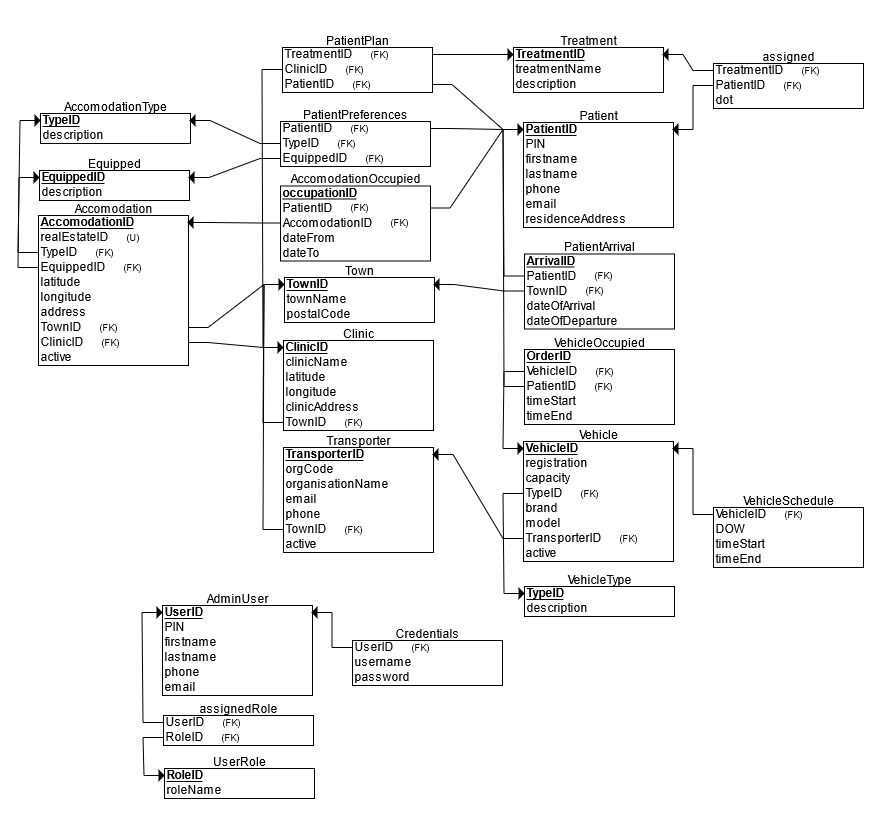
\includegraphics[width=\textwidth]{slike/DB_shema.PNG} %veličina u odnosu na širinu linije
					\caption{Sheme baze podataka}
					\label{fig:db_scheme} %label mora biti drugaciji za svaku sliku
				\end{figure}
			%Beskorisni komentar ....... :) MUAHHAHAHAH
			\eject
			
			
		\section{Dijagram razreda}
		
			Na slikama 4.2 i 4.3 su prikazani razredi \textit{Model} i \textit{Controller} iz MVC arhitekture. Razredi prikazani slikom 4.2 nasljeđuju razred Controller. Metode koje smo definirali unutar tih razreda pripremaju podatke i šalju ih bazi koja ih onda obrađuje. Baza manipulira modelima te na kraju vraća podatke kako bi ih \textit{View} mogao prikazati. Model razredi, prikazani slikom 4.3, prikazuju strukturu baze podataka te integrirane funkcije koje služe za obradu, slanje ili primanje podataka.
			
			\begin{figure}[H]
				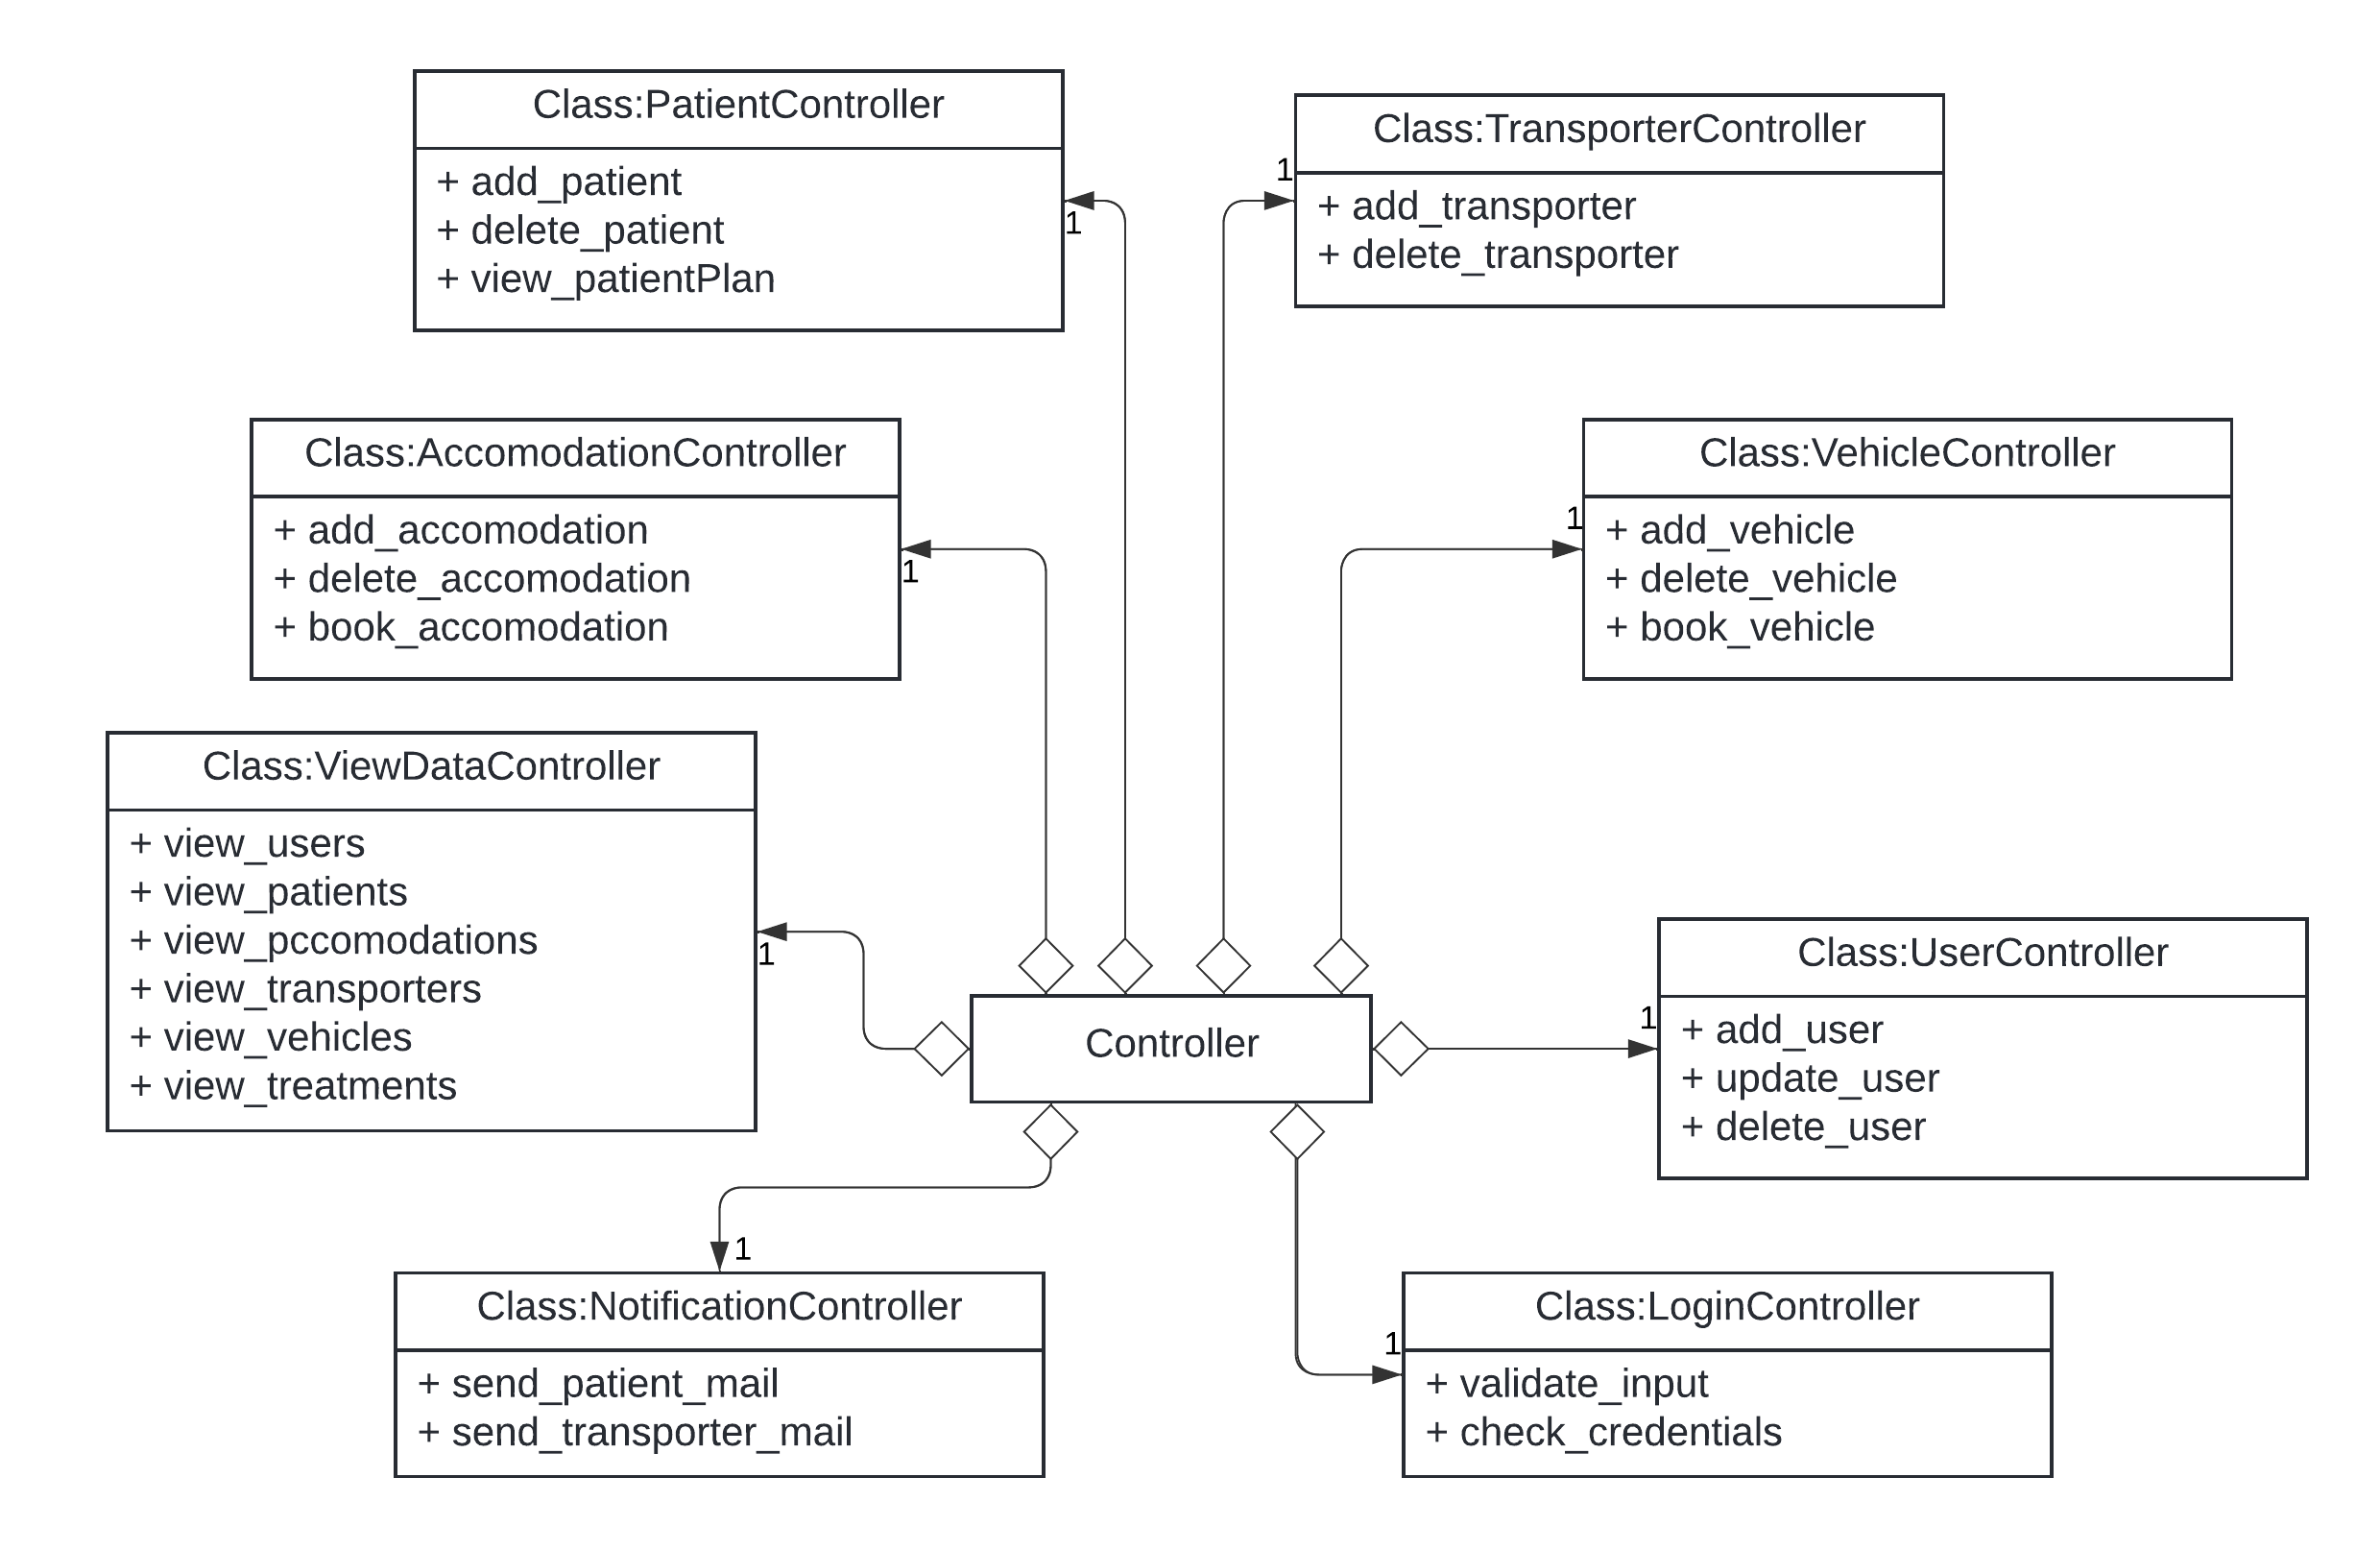
\includegraphics[width=\textwidth]{slike/UML_controller.PNG} %veličina u odnosu na širinu linije
				\caption{Dijagram razreda Controller}
				\label{fig:uml_controller} %label mora biti drugaciji za svaku sliku
			\end{figure}
			
			\begin{figure}[H]
				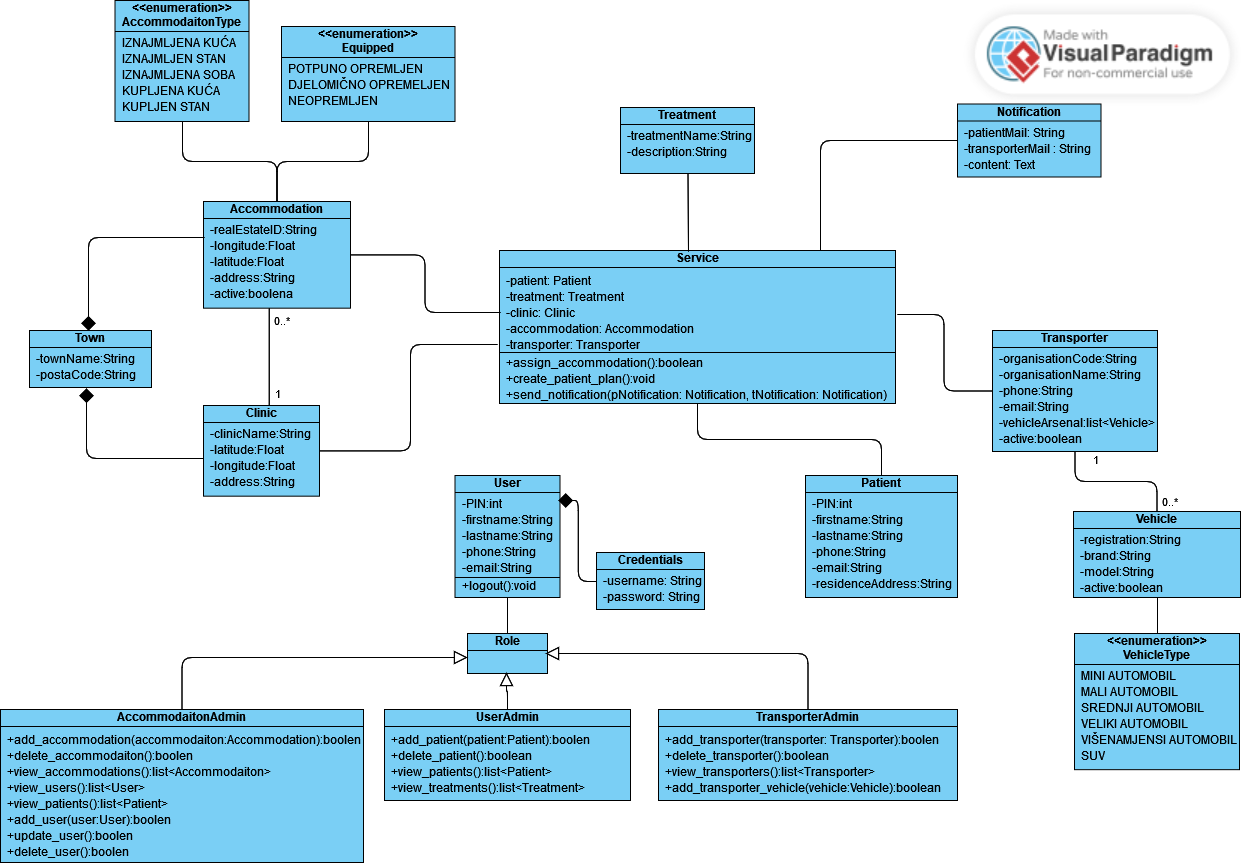
\includegraphics[width=\textwidth]{slike/UML_new_model.PNG} %veličina u odnosu na širinu linije
				\caption{Dijagram razreda Model}
				\label{fig:uml_model} %label mora biti drugaciji za svaku sliku
			\end{figure}
			
			\textbf{\textit{dio 2. revizije}}\\			
			
			\textit{Prilikom druge predaje projekta dijagram razreda i opisi moraju odgovarati stvarnom stanju implementacije}
			
			
			
			\eject
		
		\section{Dijagram stanja}
			
			
			\textbf{\textit{dio 2. revizije}}\\
			
			\textit{Potrebno je priložiti dijagram stanja i opisati ga. Dovoljan je jedan dijagram stanja koji prikazuje \textbf{značajan dio funkcionalnosti} sustava. Na primjer, stanja korisničkog sučelja i tijek korištenja neke ključne funkcionalnosti jesu značajan dio sustava, a registracija i prijava nisu. }
			
			
			\eject 
		
		\section{Dijagram aktivnosti}
			
			\textbf{\textit{dio 2. revizije}}\\
			
			 \textit{Potrebno je priložiti dijagram aktivnosti s pripadajućim opisom. Dijagram aktivnosti treba prikazivati značajan dio sustava.}
			
			\eject
		\section{Dijagram komponenti}
		
			\textbf{\textit{dio 2. revizije}}\\
		
			 \textit{Potrebno je priložiti dijagram komponenti s pripadajućim opisom. Dijagram komponenti treba prikazivati strukturu cijele aplikacije.}
	\chapter{Implementacija i korisničko sučelje}
		
		
		\section{Korištene tehnologije i alati}

			 U timu smo za vrijeme projekta komunicirali ponajviše preko aplikacija Whatts up\footnote{\url{https://www.whatsapp.com/}} te Discorda\footnote{\url{https://discord.com/}}, a sa asistentom i demonstratorom preko Microsoft Teams\footnote{\url{https://teams.microsoft.com/v2/}} i Microsoft Outlook\footnote{\url{https://outlook.office.com/mail/}}. Tekst u dokumentaciji smo uređivali pomoću latex-a\footnote{\url{https://www.latex-project.org/}} u editoru texStudio\footnote{\url{https://www.texstudio.org/}} te generirali PDF dokument iz latex dokumenta pomoću TexLive\footnote{\url{https://www.tug.org/texlive/}}. Dijagrame uporabe te sekvencijske dijagrame smo izradili pomoću alata Astah UML\footnote{\url{https://astah.net/products/astah-uml/}}.
			 
			 Nedostaje za ostale dijagrame!!!!
			 
			 Model baze podataka je napravljen pomoću alata ERDplus\footnote{\url{https://erdplus.com/}}. Kako bi smo zajedno mogli raditi na projektu u isto vrijeme te ujedno i pratiti razvojne verzije našeg projekta smo koristili Git\footnote{\url{https://git-scm.com/}} zajedno za udaljenim repozitorijom GitHub\footnote{\url{https://github.com/}}. Razvojna okruženja koja su korištena su Visual Studio Code\footnote{\url{https://code.visualstudio.com/}} te pgAdmin4\footnote{\url{https://www.pgadmin.org/}}. Frontend je napisan u programskom jezika javascript\footnote{\url{https://www.javascript.com/}} pomoću biblioteke React\footnote{\url{https://react.dev/}}, dok je za backend korišten PostgreSQL\footnote{\url{https://www.postgresql.org/}}. Unit testovi su odrađeni pomoću alata pgTAP\footnote{\url{https://pgtap.org/}}, dok su integracijski testovi napravljeni pomoću alata Selenium\footnote{\url{https://www.postgresql.org/}} i programskog  jezika Java\footnote{\url{https://www.java.com/en/}}????
			 
			 Aplikacija je puštena u pogon na servisu render\footnote{\url{https://render.com/}}.
			 
			 Fali za latex i texStudio
			
			\eject 
		
	
		\section{Ispitivanje programskog rješenja}
			
			\subsection{Ispitivanje komponenti}
				Ispitivanje jedinica je provedeno pomoću alata pgTAP. pgTAP je skup funkcija baze podataka koje olakšavaju pisanje testova. Pomoću ovog smo alata testirali izvođenje i ponašanje backenda-a ostvarenog kroz funkcije u bazi napisane plpgsql programskim jezikom. Alat nudi brojne definirane metode koje omogućuju definiranje očekivanog ispisa za određeni ulaz, uspoređivanje rezultata odrađene funkcije sa podacima iz tablica, itd.
				\eject
				\subsection{Ispitni slučaj 1 - funkcionalnost prijave}
				Ovaj ispitni slučaj ispituje funkcionalnost prijave u sustav. Testovi ispitnog slučaja testiraju postoji li funkcija u bazi, je li funkcija napisana plpgsql jezikom te koji su ulazni i izlazni tipovi podataka funkcije. To se testira koristeći ugrađene funkcije pgTAP-a kao što su \textit{\texttt{has\_function}} za testiranje postoji li definirana funkcija u bazi, \textit{\texttt{function\_lang\_is}} za testiranje je li funkcija napisana plpgsql jezikom, \textit{\texttt{function\_returns}} za testiranje vraća li funkcija neki tip podataka ili je tipa void, \textit{\texttt{is\(\)}} ze provjeru dvaju argumenata te na osnovu njihovog podudaranje ili odudaranja se izbacuje rezultat. Rezultat je uvijek u obliku jednog reda sa jednom kolonom koja može sadržavati tekst \textit{ok $<$broj testa$>$ - $<$opis testa$>$} ili \textit{not ok $<$broj testa$>$ - $<$opis testa$>$}.
				\begin{figure}[H]
					\centering
					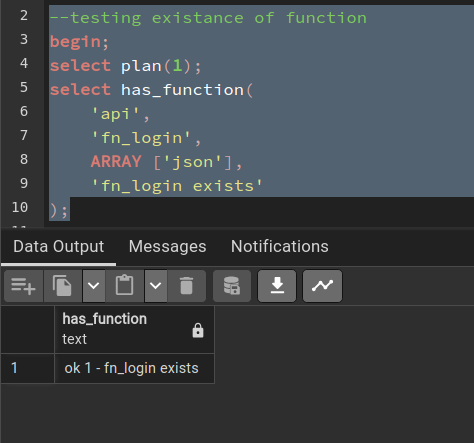
\includegraphics[width=\textwidth]{slike/unit_tests/ut_1/has_func.png}
					\caption{Pokretanje testa za provjeru postojanja funkcije}
					\label{fig: IS1-has_function}
				\end{figure}
				\begin{figure}[H]
					\centering
					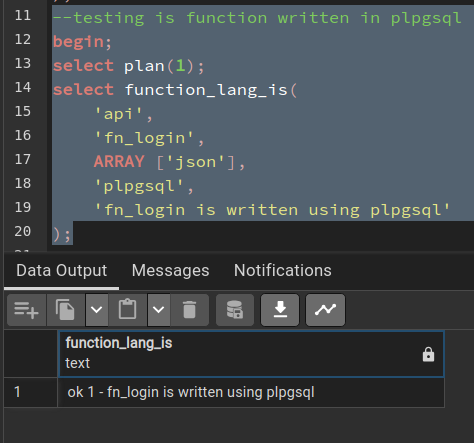
\includegraphics[width=\textwidth]{slike/unit_tests/ut_1/func_lang.png}
					\caption{Pokretanje testa za provjeru jezika kojim je napisana funkcija}
					\label{fig: IS1-function_lang}
				\end{figure}
				\begin{figure}[H]
					\centering
					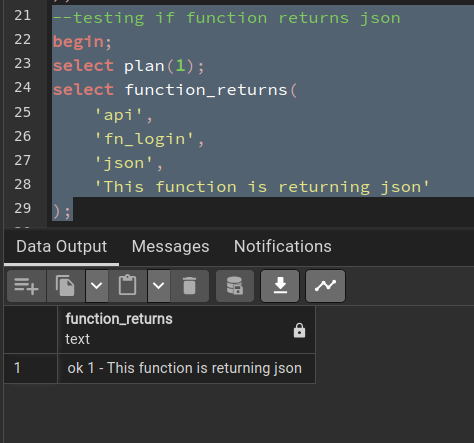
\includegraphics[width=\textwidth]{slike/unit_tests/ut_1/func_return.png}
					\caption{Pokretanje testa za provjeru povratnog tipa podatka funkcije}
					\label{fig: IS1-function_return}
				\end{figure}
				\begin{figure}[H]
					\centering
					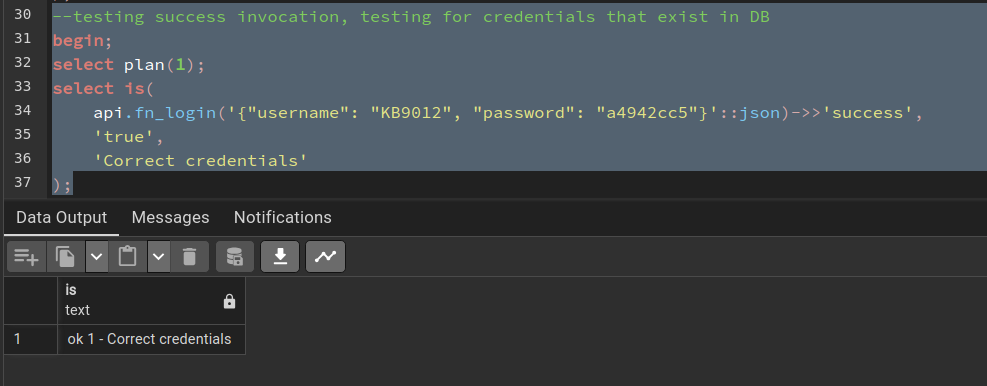
\includegraphics[width=\textwidth]{slike/unit_tests/ut_1/success_login.png}
					\caption{Pokretanje testa za provjeru rada same funkcije, uspijeh}
					\label{fig: IS1-uspješni login}
				\end{figure}
				\begin{figure}[H]
					\centering
					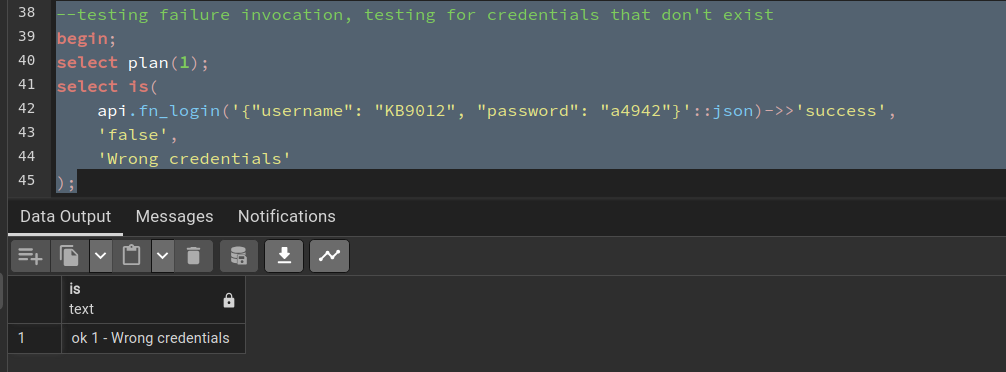
\includegraphics[width=\textwidth]{slike/unit_tests/ut_1/failure_login.png}
					\caption{Pokretanje testa za provjeru rada same funkcije, neuspijeh}
					\label{fig: IS1-neuspješni login}
				\end{figure}
				\begin{figure}[H]
					\centering
					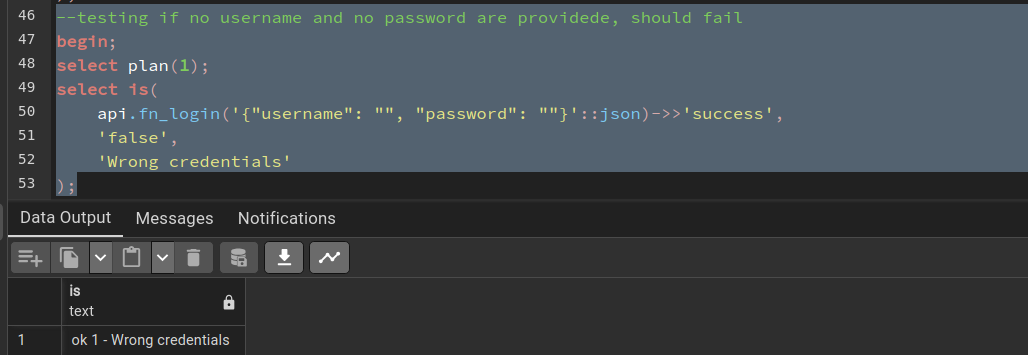
\includegraphics[width=\textwidth]{slike/unit_tests/ut_1/no_creds.png}
					\caption{Pokretanje testa za provjeru rada same funkcije, neuspijeh}
					\label{fig: IS1-login bez vjerodajnica}
				\end{figure}
				\begin{figure}[H]
					\centering
					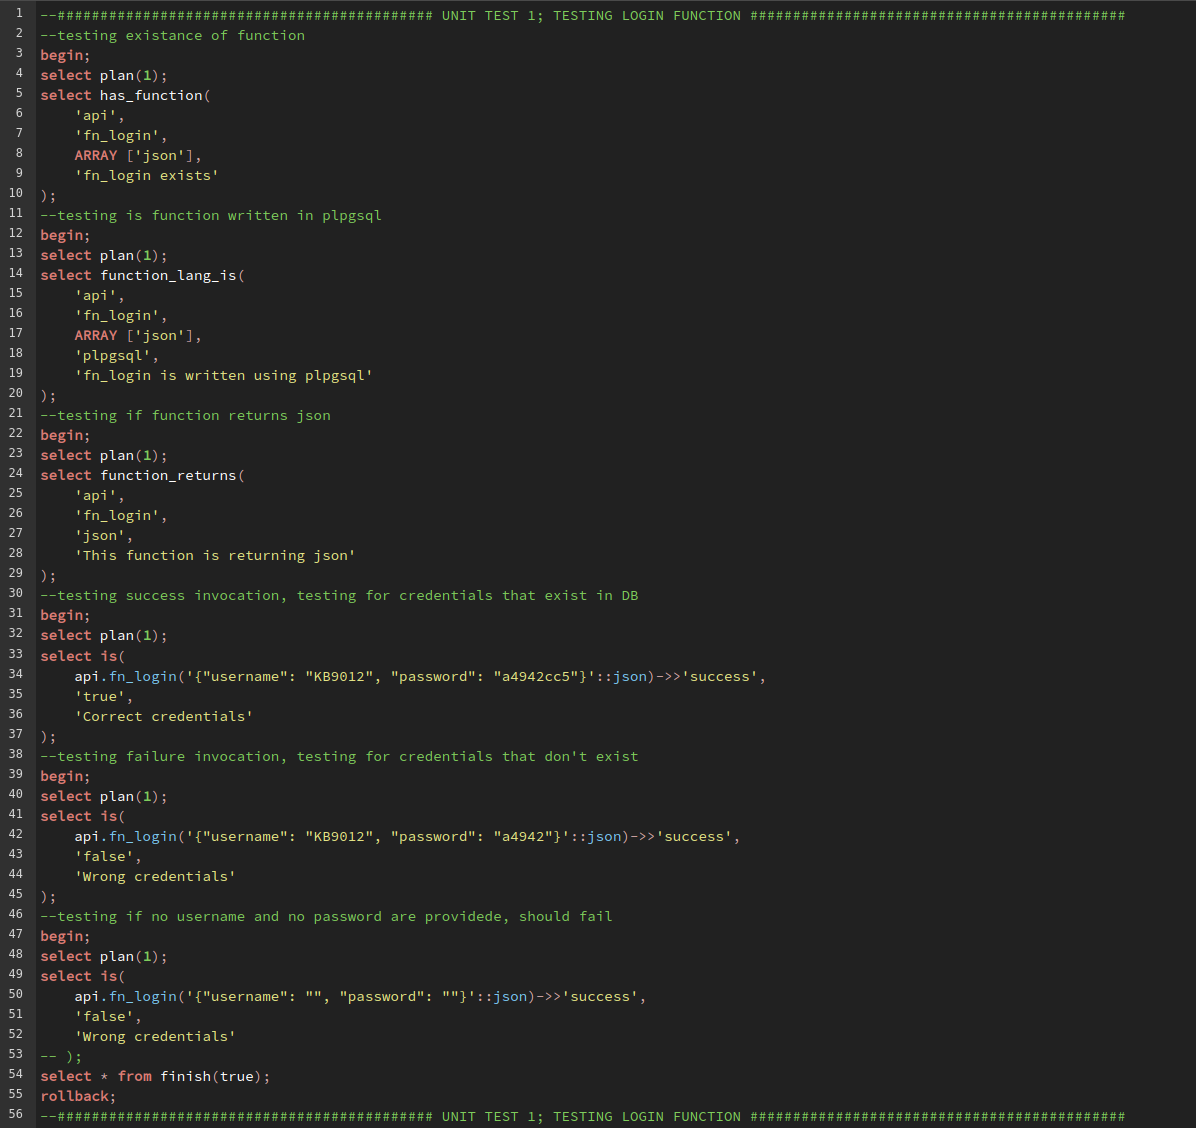
\includegraphics[width=\textwidth]{slike/unit_tests/ut_1/code.png}
					\caption{Kod isptinog slučaja 1}
					\label{fig: IS1-kod}
				\end{figure}
				\eject
				\subsection{Ispitni slučaj 2 - funkcionalnost dodavanja novog administratora}
				Ovaj ispitni slučaj ispituje funkcionalnost dodavanja novog administratora. Testovi ispitnog slučaja testiraju postoji li funkcija u bazi, je li funkcija napisana plpgsql jezikom te koji su ulazni i izlazni tipovi podataka funkcije. To se testira koristeći ugrađene funkcije pgTAP-a kao što su \textit{\texttt{has\_function}} za testiranje postoji li definirana funkcija u bazi, \textit{\texttt{function\_lang\_is}} za testiranje je li funkcija napisana plpgsql jezikom, \textit{\texttt{function\_returns}} za testiranje vraća li funkcija neki tip podataka ili je tipa void, \textit{\texttt{is\(\)}} ze provjeru dvaju argumenata te na osnovu njihovog podudaranje ili odudaranja se izbacuje rezultat. Rezultat je uvijek u obliku jednog reda sa jednom kolonom koja može sadržavati tekst \textit{ok $<$broj testa$>$ - $<$opis testa$>$} ili \textit{not ok $<$broj testa$>$ - $<$opis testa$>$}.
				\begin{figure}[H]
					\centering
					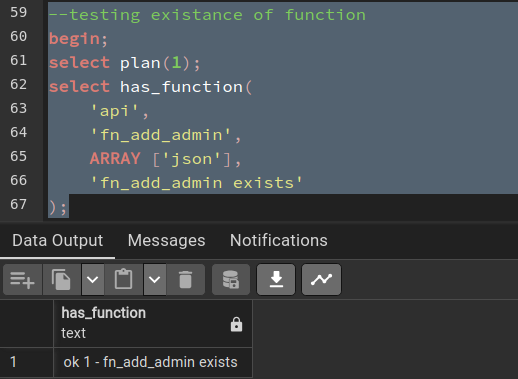
\includegraphics[width=\textwidth]{slike/unit_tests/ut_2/has_func.png}
					\caption{Pokretanje testa za provjeru postojanja funkcije}
					\label{fig: IS2-has_function}
				\end{figure}
				\begin{figure}[H]
					\centering
					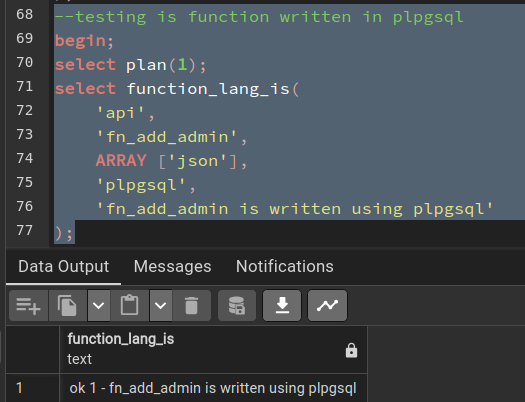
\includegraphics[width=\textwidth]{slike/unit_tests/ut_2/func_lang.png}
					\caption{Pokretanje testa za provjeru jezika kojim je napisana funkcija}
					\label{fig: IS2-function_lang}
				\end{figure}
				\begin{figure}[H]
					\centering
					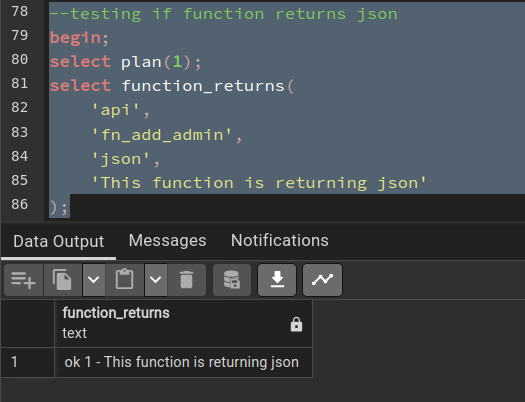
\includegraphics[width=\textwidth]{slike/unit_tests/ut_2/func_return.png}
					\caption{Pokretanje testa za provjeru povratnog tipa podatka funkcije}
					\label{fig: IS2-function_return}
				\end{figure}
				\begin{figure}[H]
					\centering
					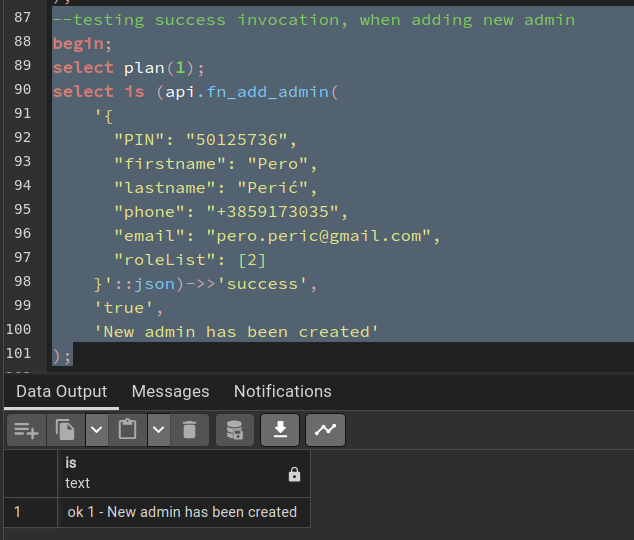
\includegraphics[width=\textwidth]{slike/unit_tests/ut_2/success_invocation.png}
					\caption{Pokretanje testa za provjeru rada same funkcije, uspijeh}
					\label{fig: IS2-uspješno kreiran administrator}
				\end{figure}
				\begin{figure}[H]
					\centering
					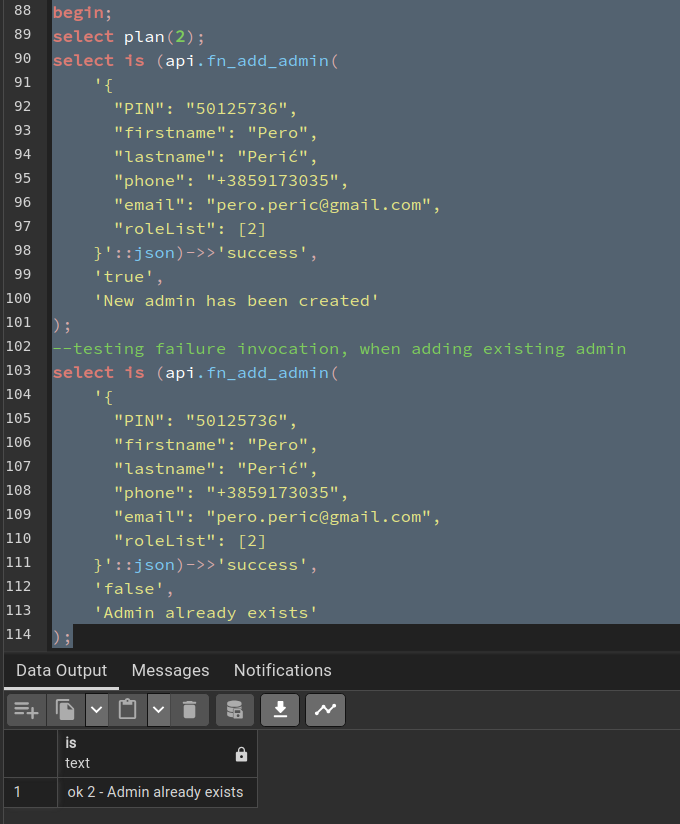
\includegraphics[width=\textwidth]{slike/unit_tests/ut_2/failure_invocation.png}
					\caption{Pokretanje testa za provjeru rada same funkcije, neuspijeh}
					\label{fig: IS2-administrator nije kreiran, već postoji isti}
				\end{figure}
				\begin{figure}[H]
					\centering
					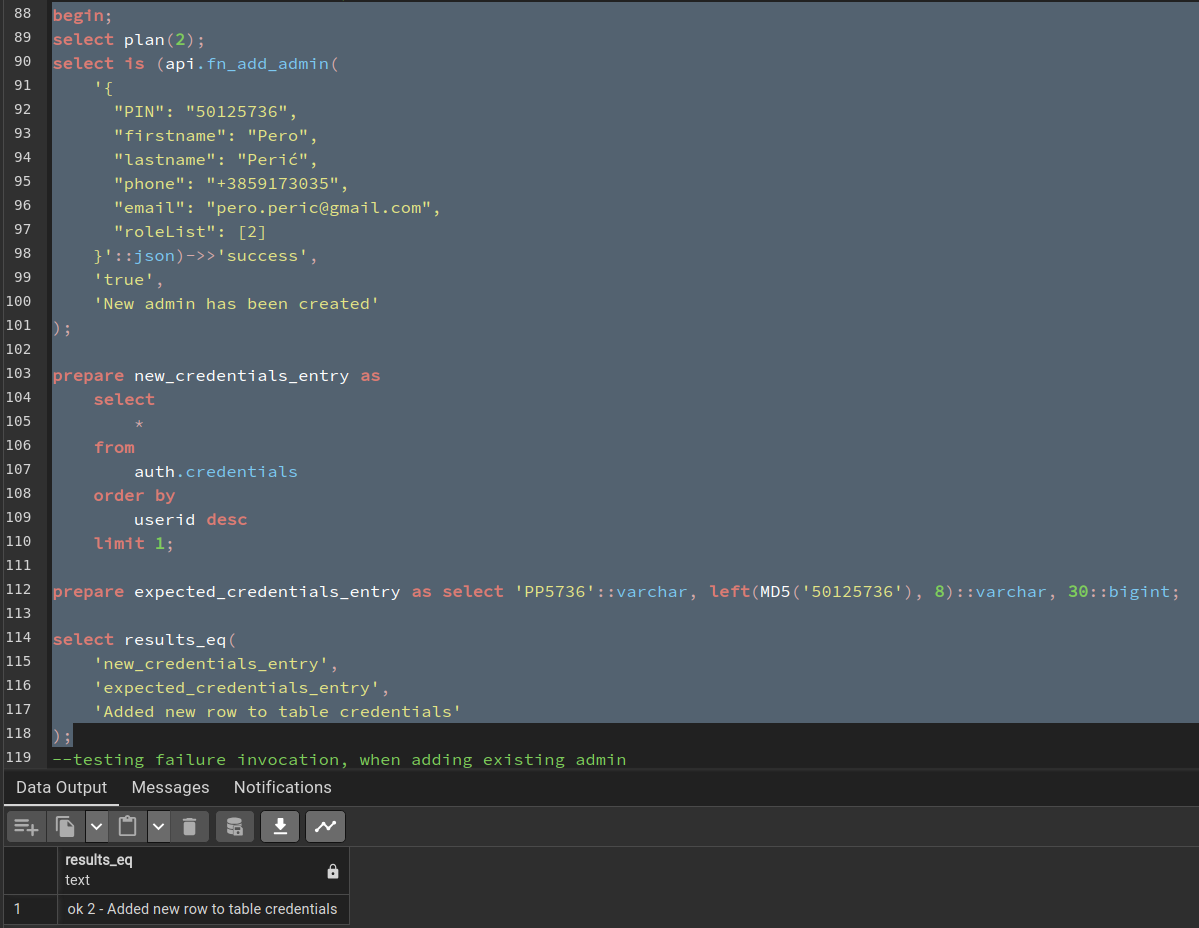
\includegraphics[width=\textwidth]{slike/unit_tests/ut_2/credentials_creation.png}
					\caption{Pokretanje testa za provjeru automatskog kreiranja vjerodajnica za novog administratora}
					\label{fig: IS2-kreirane vjerodajnice za novod administratora}
				\end{figure}
				\begin{figure}[H]
					\centering
					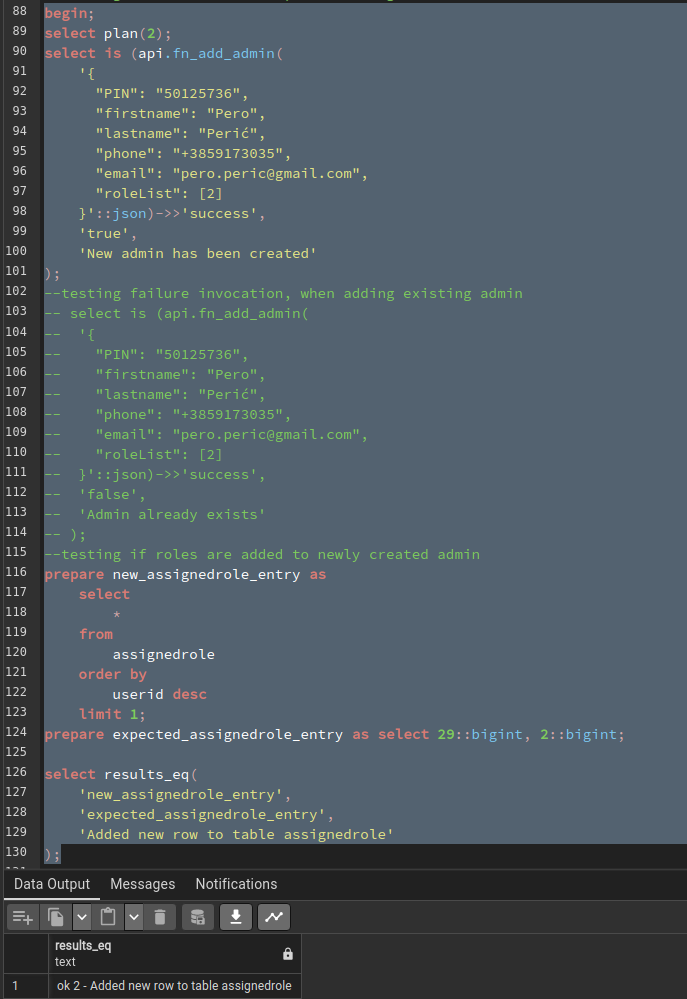
\includegraphics[width=\textwidth]{slike/unit_tests/ut_2/role_assigned.png}
					\caption{Pokretanje testa za provjeru automatskog dodjeljivanja uloge/uloga za novog administratora}
					\label{fig: IS2-dodavanje uloga novom adminstratoru}
				\end{figure}
				\begin{figure}[H]
					\centering
					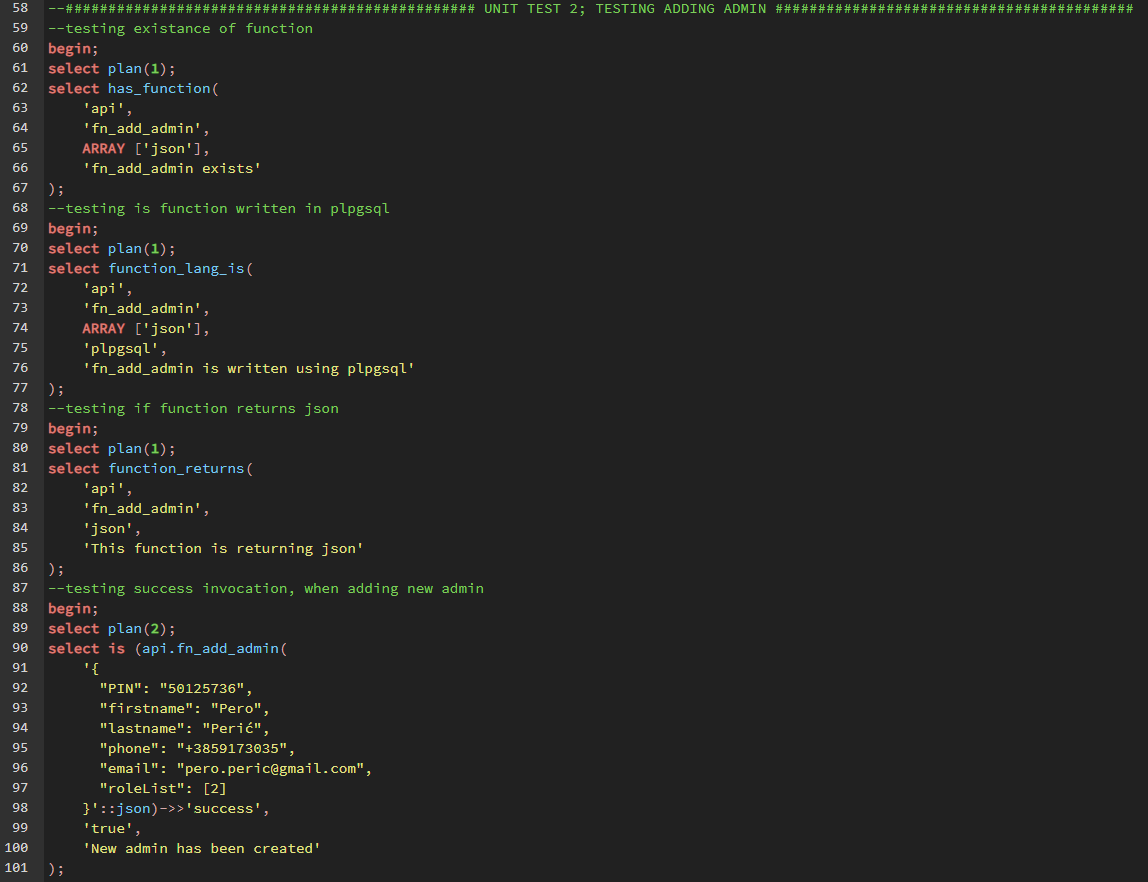
\includegraphics[width=\textwidth]{slike/unit_tests/ut_2/code_part1.png}
					\label{fig: IS2-code part 1}
				\end{figure}
				\begin{figure}[H]
					\centering
					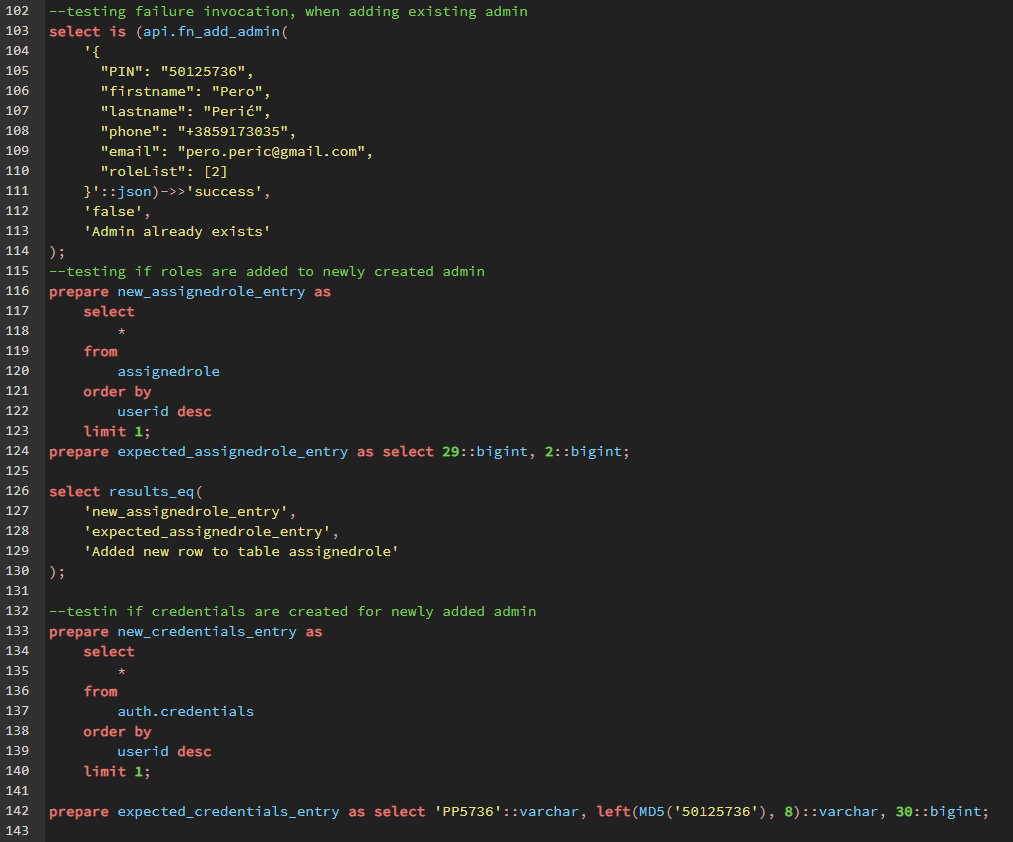
\includegraphics[width=\textwidth]{slike/unit_tests/ut_2/code_part2.png}
					\label{fig: IS2-code part 2}
				\end{figure}
				\begin{figure}[H]
					\centering
					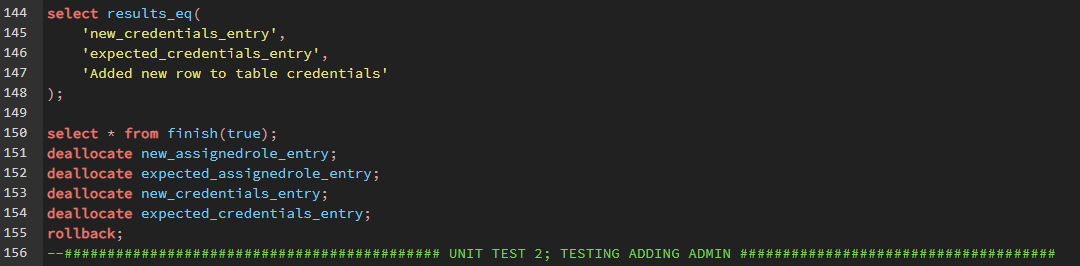
\includegraphics[width=\textwidth]{slike/unit_tests/ut_2/code_part3.png}
					\caption{Kod ispitnog slučaja 2}
					\label{fig: IS2-code part 3}
				\end{figure}
				\eject
				\subsection{Ispitni slučaj 3 - funkcionalnost brisanja administratora}
				Ovaj ispitni slučaj ispituje funkcionalnost brisanja administratora. Testovi ispitnog slučaja testiraju postoji li funkcija u bazi, je li funkcija napisana plpgsql jezikom te koji su ulazni i izlazni tipovi podataka funkcije. To se testira koristeći ugrađene funkcije pgTAP-a kao što su \textit{\texttt{has\_function}} za testiranje postoji li definirana funkcija u bazi, \textit{\texttt{function\_lang\_is}} za testiranje je li funkcija napisana plpgsql jezikom, \textit{\texttt{function\_returns}} za testiranje vraća li funkcija neki tip podataka ili je tipa void, \textit{\texttt{is\(\)}} ze provjeru dvaju argumenata te na osnovu njihovog podudaranje ili odudaranja se izbacuje rezultat. Rezultat je uvijek u obliku jednog reda sa jednom kolonom koja može sadržavati tekst \textit{ok $<$broj testa$>$ - $<$opis testa$>$} ili \textit{not ok $<$broj testa$>$ - $<$opis testa$>$}.
				\begin{figure}[H]
					\centering
					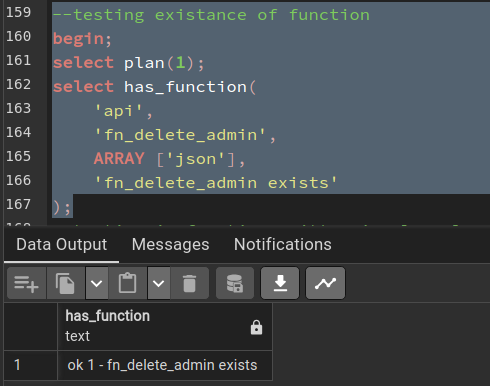
\includegraphics[width=\textwidth]{slike/unit_tests/ut_3/has_func.png}
					\caption{Pokretanje testa za provjeru postojanja funkcije}
					\label{fig: IS3-has_function}
				\end{figure}
				\begin{figure}[H]
					\centering
					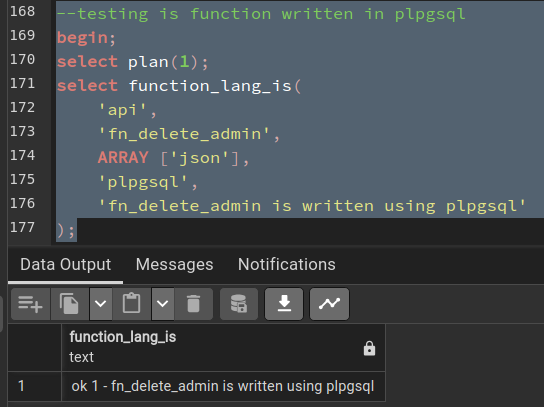
\includegraphics[width=\textwidth]{slike/unit_tests/ut_3/func_lang.png}
					\caption{Pokretanje testa za provjeru jezika kojim je napisana funkcija}
					\label{fig: IS3-function_lang}
				\end{figure}
				\begin{figure}[H]
					\centering
					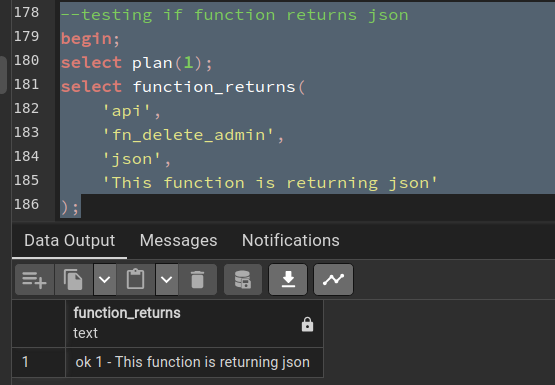
\includegraphics[width=\textwidth]{slike/unit_tests/ut_3/func_return.png}
					\caption{Pokretanje testa za provjeru povratnog tipa podatka funkcije}
					\label{fig: IS3-function_return}
				\end{figure}
				\begin{figure}[H]
					\centering
					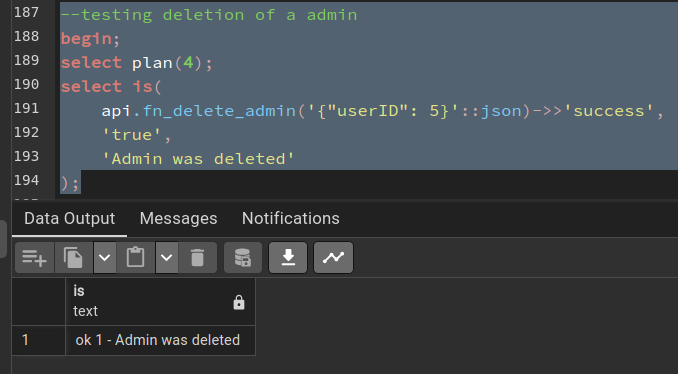
\includegraphics[width=\textwidth]{slike/unit_tests/ut_3/success_invocation.png}
					\caption{Pokretanje testa za provjeru rada same funkcije, uspijeh}
					\label{fig: IS3-uspješno izbrisan administrator}
				\end{figure}
				\begin{figure}[H]
					\centering
					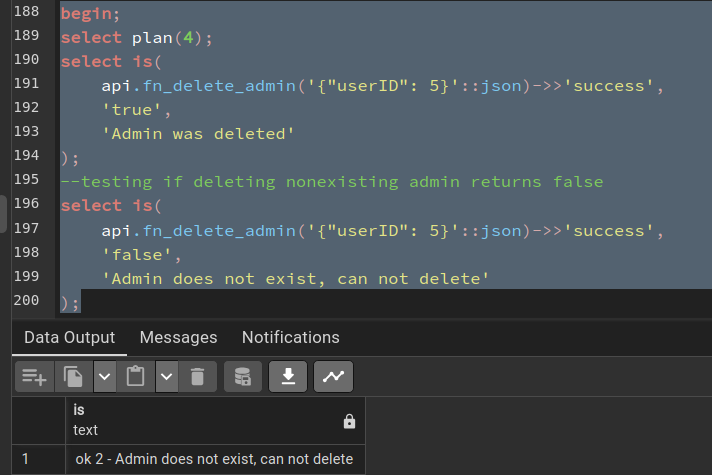
\includegraphics[width=\textwidth]{slike/unit_tests/ut_3/failure_invocation.png}
					\caption{Pokretanje testa za provjeru rada same funkcije, neuspijeh}
					\label{fig: IS3-administrator je već izbrisan ili ne postoji}
				\end{figure}
				\begin{figure}[H]
					\centering
					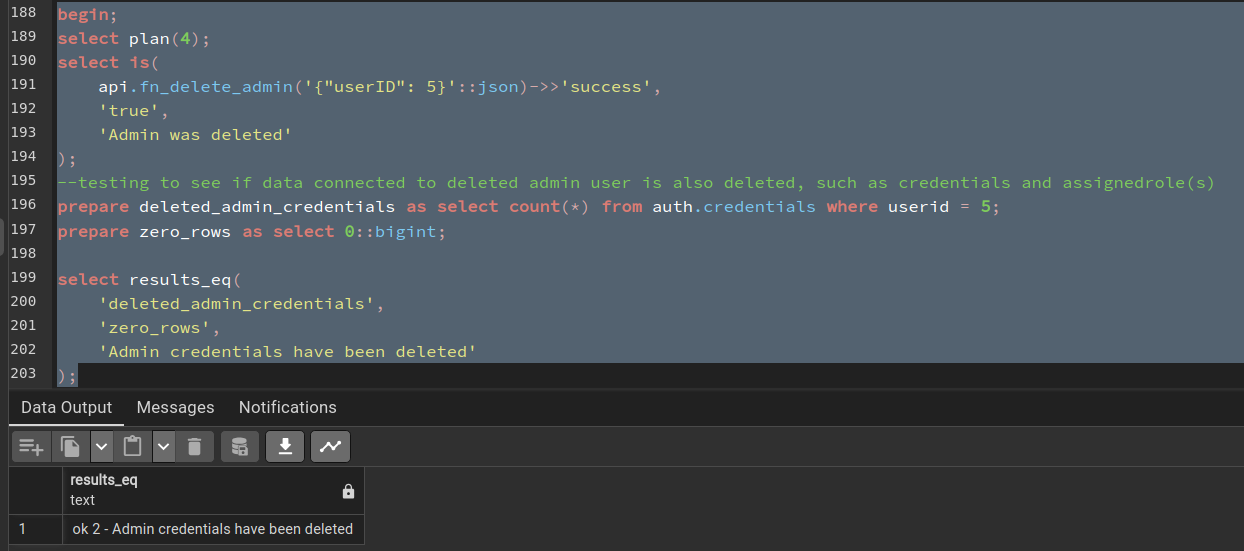
\includegraphics[width=\textwidth]{slike/unit_tests/ut_3/credentials_deletion.png}
					\caption{Pokretanje testa za provjeru automatskog brisanja vjerodajnica za izbrisanog administratora}
					\label{fig: IS3-brisanje vjerodajnice za obrisanog administratora}
				\end{figure}
				\begin{figure}[H]
					\centering
					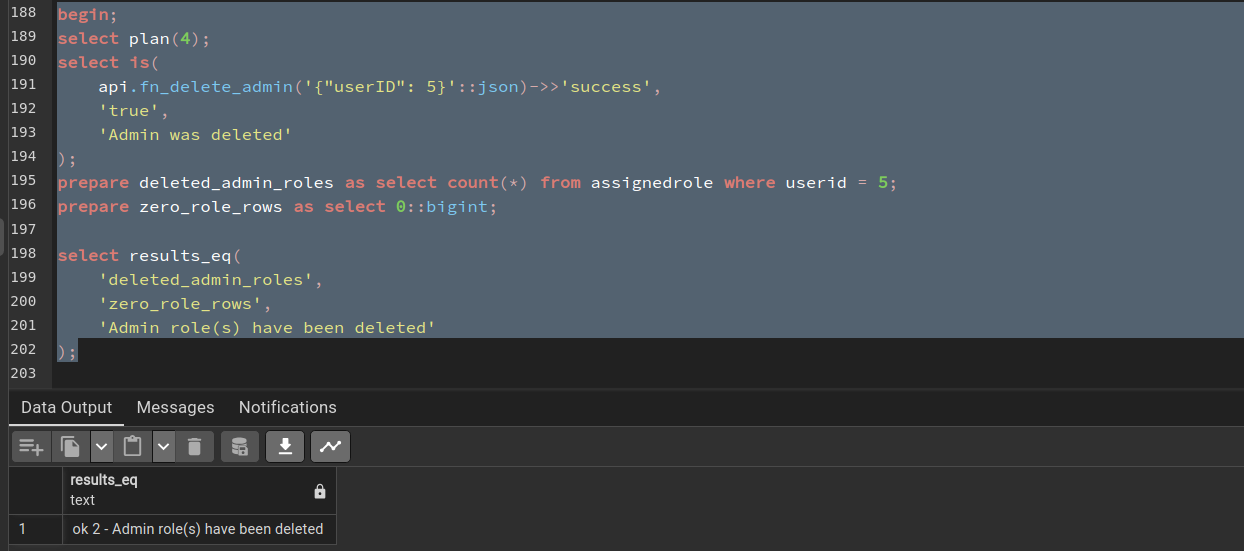
\includegraphics[width=\textwidth]{slike/unit_tests/ut_3/role_deletion.png}
					\caption{Pokretanje testa za provjeru automatskog brisanja pridjeljenih uloga za obrisanog administratora}
					\label{fig: IS3-brisanje pridjeljenih uloga za obrisanog administratora}
				\end{figure}
				\begin{figure}[H]
					\centering
					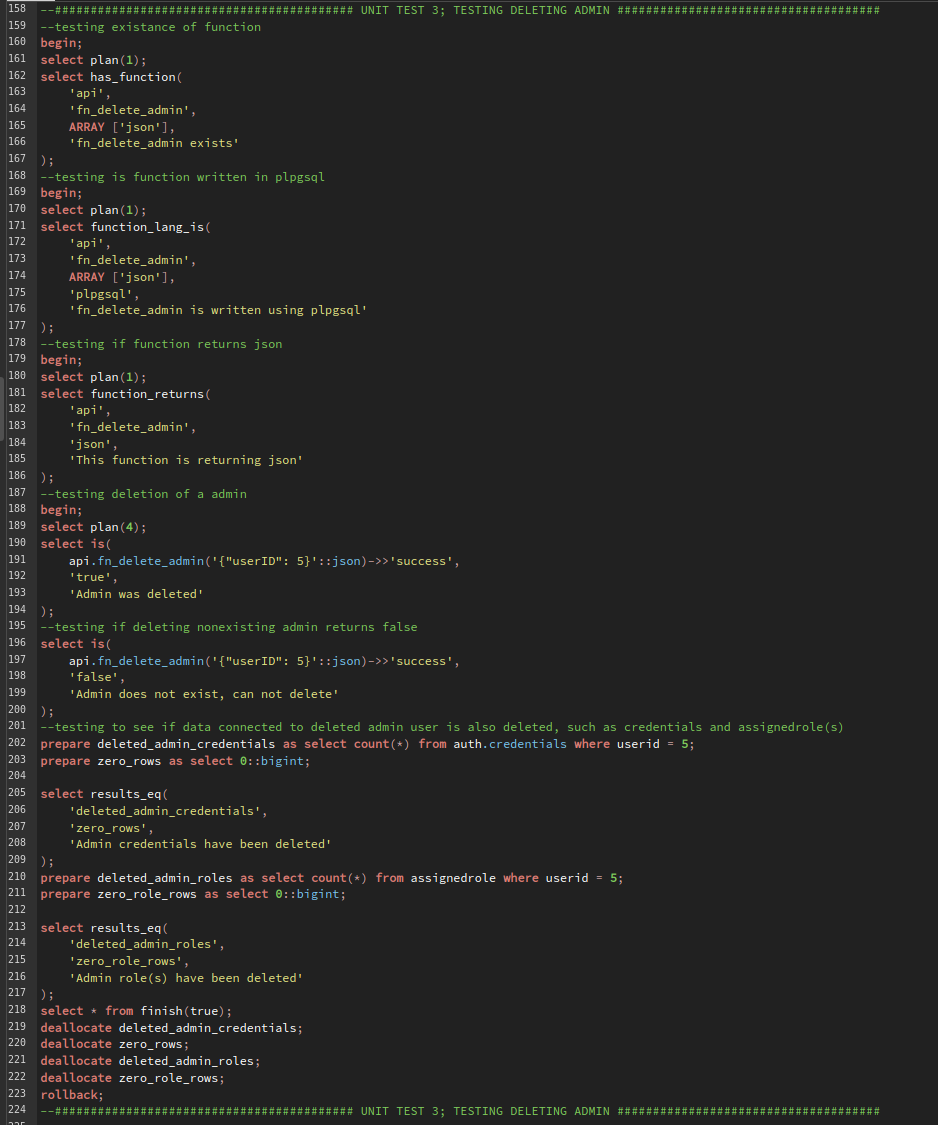
\includegraphics[width=\textwidth]{slike/unit_tests/ut_3/code.png}
					\caption{Kod isptinog slučaja 3}
					\label{fig: IS3-kod}
				\end{figure}
				\eject
				\subsection{Ispitni slučaj 4 - funkcionalnost dodavanja smještaja}
				Ovaj ispitni slučaj ispituje funkcionalnost dodavanja smještaja. Testovi ispitnog slučaja testiraju postoji li funkcija u bazi, je li funkcija napisana plpgsql jezikom te koji su ulazni i izlazni tipovi podataka funkcije. To se testira koristeći ugrađene funkcije pgTAP-a kao što su \textit{\texttt{has\_function}} za testiranje postoji li definirana funkcija u bazi, \textit{\texttt{function\_lang\_is}} za testiranje je li funkcija napisana plpgsql jezikom, \textit{\texttt{function\_returns}} za testiranje vraća li funkcija neki tip podataka ili je tipa void, \textit{\texttt{is\(\)}} ze provjeru dvaju argumenata te na osnovu njihovog podudaranje ili odudaranja se izbacuje rezultat. Rezultat je uvijek u obliku jednog reda sa jednom kolonom koja može sadržavati tekst \textit{ok $<$broj testa$>$ - $<$opis testa$>$} ili \textit{not ok $<$broj testa$>$ - $<$opis testa$>$}.
				\begin{figure}[H]
					\centering
					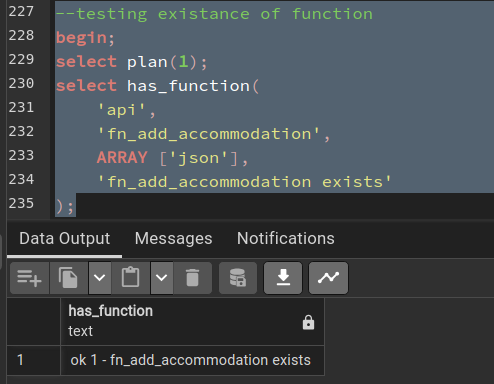
\includegraphics[width=\textwidth]{slike/unit_tests/ut_4/has_func.png}
					\caption{Pokretanje testa za provjeru postojanja funkcije}
					\label{fig: IS4-has_function}
				\end{figure}
				\begin{figure}[H]
					\centering
					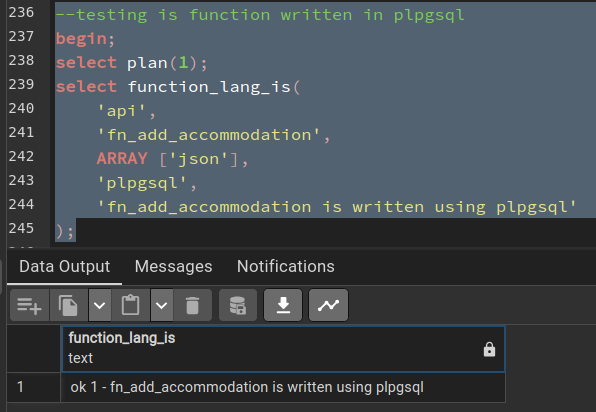
\includegraphics[width=\textwidth]{slike/unit_tests/ut_4/func_lang.png}
					\caption{Pokretanje testa za provjeru jezika kojim je napisana funkcija}
					\label{fig: IS4-function_lang}
				\end{figure}
				\begin{figure}[H]
					\centering
					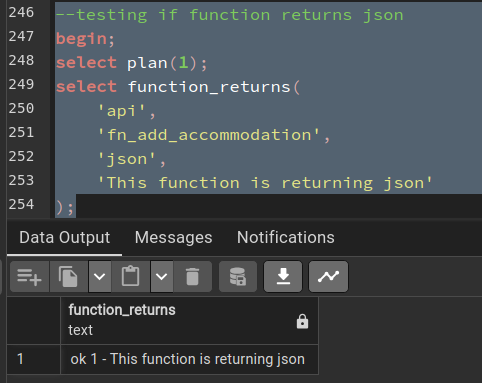
\includegraphics[width=\textwidth]{slike/unit_tests/ut_4/func_return.png}
					\caption{Pokretanje testa za provjeru povratnog tipa podatka funkcije}
					\label{fig: IS4-function_return}
				\end{figure}
				\begin{figure}[H]
					\centering
					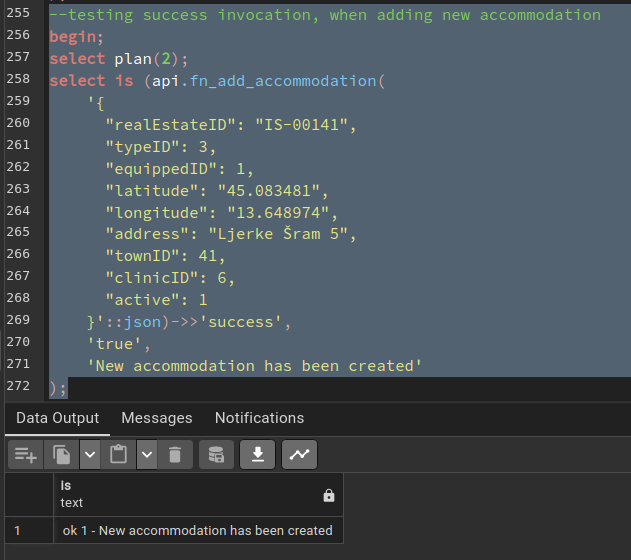
\includegraphics[width=\textwidth]{slike/unit_tests/ut_4/success_invocation.png}
					\caption{Pokretanje testa za provjeru rada same funkcije, uspijeh}
					\label{fig: IS4-uspješno kreiran smještaj}
				\end{figure}
				\begin{figure}[H]
					\centering
					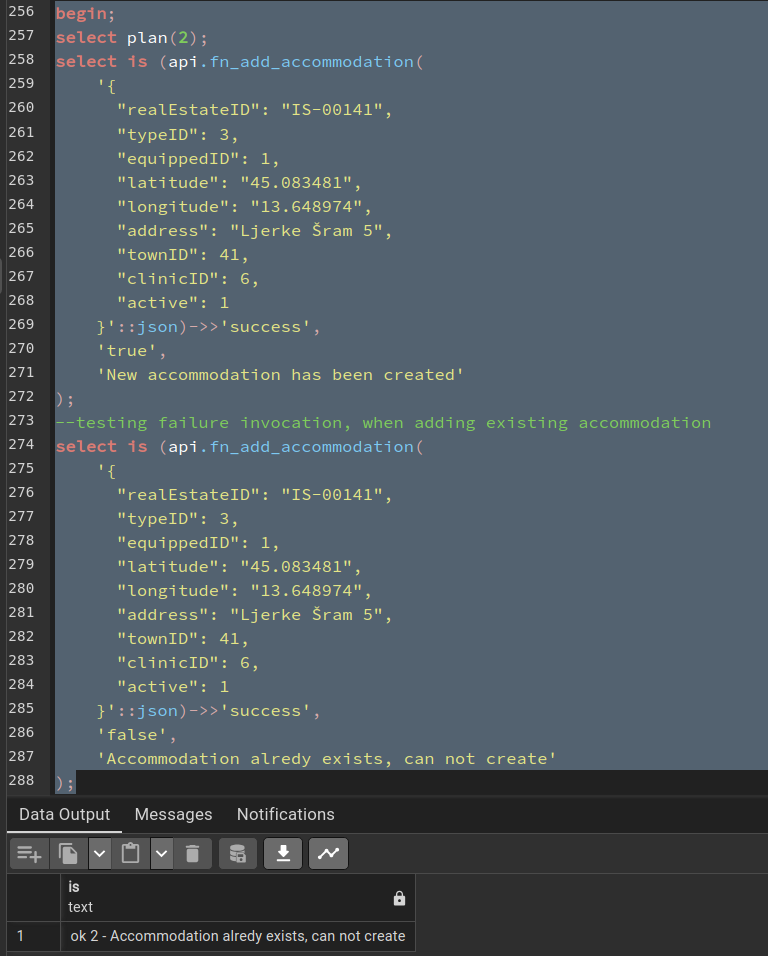
\includegraphics[width=\textwidth]{slike/unit_tests/ut_4/failure_invocation.png}
					\caption{Pokretanje testa za provjeru rada same funkcije, neuspijeh}
					\label{fig: IS4-smještaj nije kreiran, već postoji isti}
				\end{figure}
				\begin{figure}[H]
					\centering
					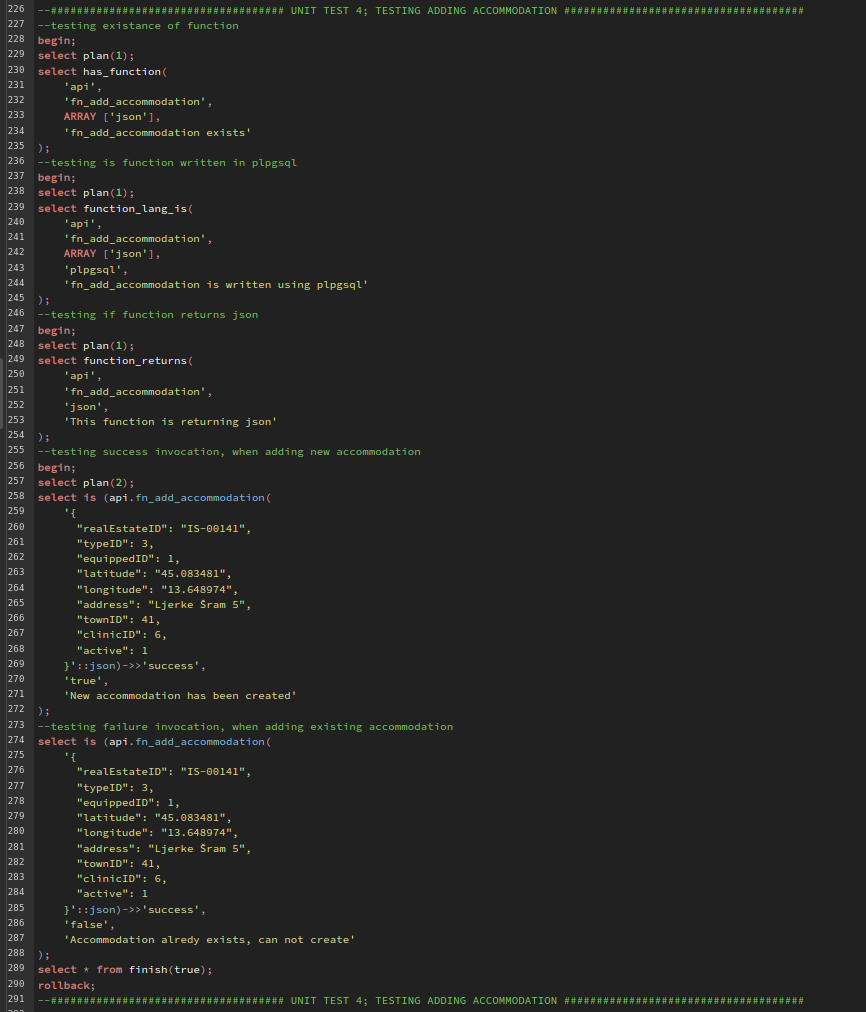
\includegraphics[width=\textwidth]{slike/unit_tests/ut_4/code.png}
					\caption{Kod isptinog slučaja 4}
					\label{fig: IS4-kod}
				\end{figure}
				\eject
				\subsection{Ispitni slučaj 5 - funkcionalnost brisanja smještaja}
				Ovaj ispitni slučaj ispituje funkcionalnost brisanja smještaja. Testovi ispitnog slučaja testiraju postoji li funkcija u bazi, je li funkcija napisana plpgsql jezikom te koji su ulazni i izlazni tipovi podataka funkcije. To se testira koristeći ugrađene funkcije pgTAP-a kao što su \textit{\texttt{has\_function}} za testiranje postoji li definirana funkcija u bazi, \textit{\texttt{function\_lang\_is}} za testiranje je li funkcija napisana plpgsql jezikom, \textit{\texttt{function\_returns}} za testiranje vraća li funkcija neki tip podataka ili je tipa void, \textit{\texttt{is\(\)}} ze provjeru dvaju argumenata te na osnovu njihovog podudaranje ili odudaranja se izbacuje rezultat. Rezultat je uvijek u obliku jednog reda sa jednom kolonom koja može sadržavati tekst \textit{ok $<$broj testa$>$ - $<$opis testa$>$} ili \textit{not ok $<$broj testa$>$ - $<$opis testa$>$}.
				\begin{figure}[H]
					\centering
					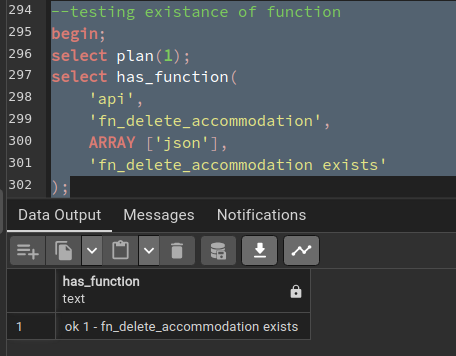
\includegraphics[width=\textwidth]{slike/unit_tests/ut_5/has_func.png}
					\caption{Pokretanje testa za provjeru postojanja funkcije}
					\label{fig: IS5-has_function}
				\end{figure}
				\begin{figure}[H]
					\centering
					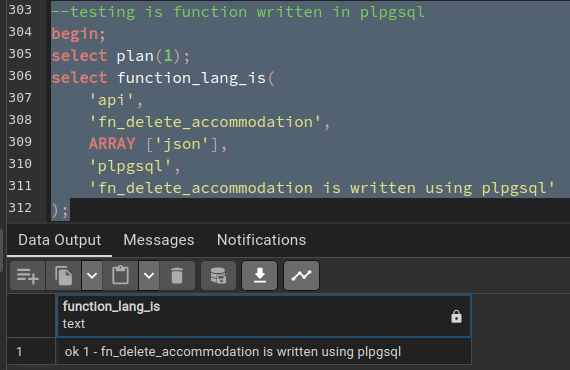
\includegraphics[width=\textwidth]{slike/unit_tests/ut_5/func_lang.png}
					\caption{Pokretanje testa za provjeru jezika kojim je napisana funkcija}
					\label{fig: IS5-function_lang}
				\end{figure}
				\begin{figure}[H]
					\centering
					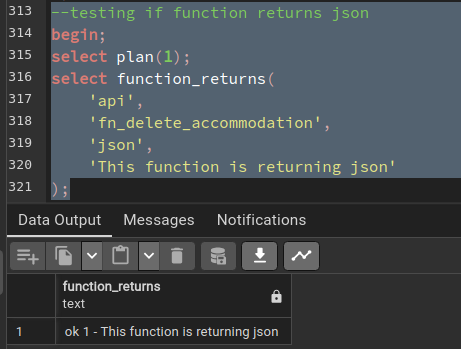
\includegraphics[width=\textwidth]{slike/unit_tests/ut_5/func_return.png}
					\caption{Pokretanje testa za provjeru povratnog tipa podatka funkcije}
					\label{fig: IS5-function_return}
				\end{figure}
				\begin{figure}[H]
					\centering
					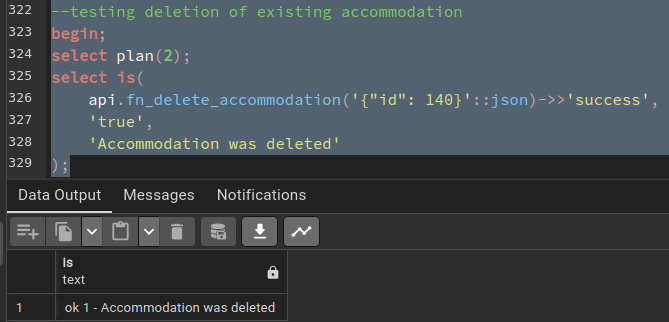
\includegraphics[width=\textwidth]{slike/unit_tests/ut_5/success_invocation.png}
					\caption{Pokretanje testa za provjeru rada same funkcije, uspijeh}
					\label{fig: IS5-uspješno izbrisan smještaj}
				\end{figure}
				\begin{figure}[H]
					\centering
					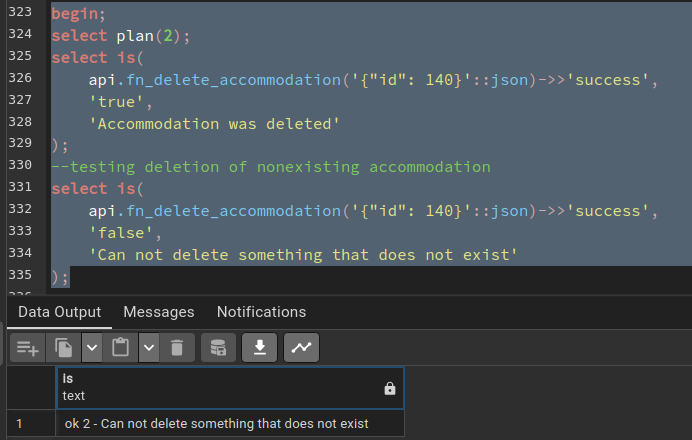
\includegraphics[width=\textwidth]{slike/unit_tests/ut_5/failure_invocation.png}
					\caption{Pokretanje testa za provjeru rada same funkcije, neuspijeh}
					\label{fig: IS5-smještaj je već izbrisan ili ne postoji}
				\end{figure}
				\begin{figure}[H]
					\centering
					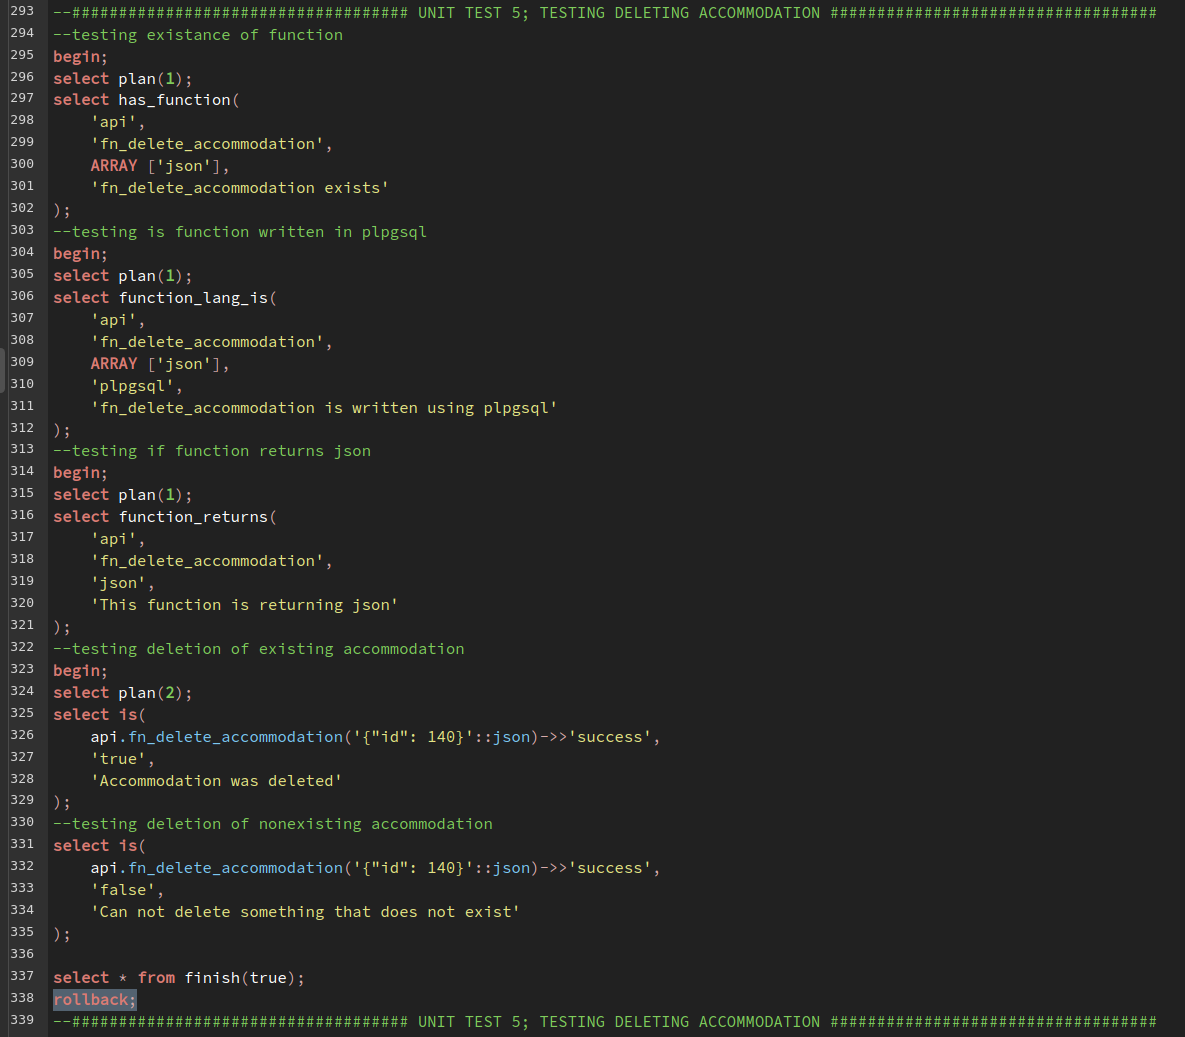
\includegraphics[width=\textwidth]{slike/unit_tests/ut_5/code.png}
					\caption{Kod isptinog slučaja 5}
					\label{fig: IS5-kod}
				\end{figure}
				\eject
				\subsection{Ispitni slučaj 6 - funkcionalnost dohvaćanja posljednjeg unesenog realestateid-a}
				Ovaj ispitni slučaj ispituje funkcionalnost dohvaćanja posljednjeg unesenog realestateid-a. Testovi ispitnog slučaja testiraju postoji li funkcija u bazi, je li funkcija napisana plpgsql jezikom te koji su ulazni i izlazni tipovi podataka funkcije. To se testira koristeći ugrađene funkcije pgTAP-a kao što su \textit{\texttt{has\_function}} za testiranje postoji li definirana funkcija u bazi, \textit{\texttt{function\_lang\_is}} za testiranje je li funkcija napisana plpgsql jezikom, \textit{\texttt{function\_returns}} za testiranje vraća li funkcija neki tip podataka ili je tipa void, \textit{\texttt{is\(\)}} ze provjeru dvaju argumenata te na osnovu njihovog podudaranje ili odudaranja se izbacuje rezultat. Rezultat je uvijek u obliku jednog reda sa jednom kolonom koja može sadržavati tekst \textit{ok $<$broj testa$>$ - $<$opis testa$>$} ili \textit{not ok $<$broj testa$>$ - $<$opis testa$>$}.
				\begin{figure}[H]
					\centering
					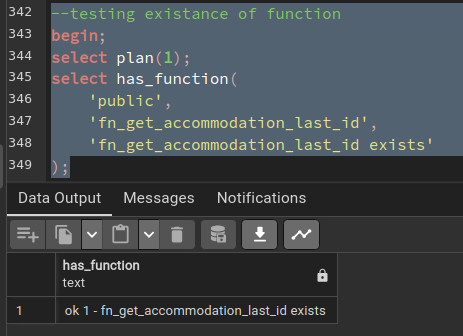
\includegraphics[width=\textwidth]{slike/unit_tests/ut_6/has_func.png}
					\caption{Pokretanje testa za provjeru postojanja funkcije}
					\label{fig: IS6-has_function}
				\end{figure}
				\begin{figure}[H]
					\centering
					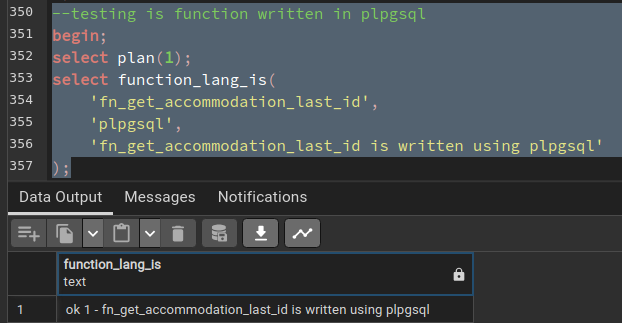
\includegraphics[width=\textwidth]{slike/unit_tests/ut_6/func_lang.png}
					\caption{Pokretanje testa za provjeru jezika kojim je napisana funkcija}
					\label{fig: IS6-function_lang}
				\end{figure}
				\begin{figure}[H]
					\centering
					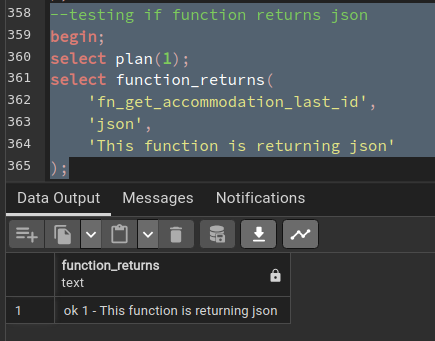
\includegraphics[width=\textwidth]{slike/unit_tests/ut_6/func_return.png}
					\caption{Pokretanje testa za provjeru povratnog tipa podatka funkcije}
					\label{fig: IS6-function_return}
				\end{figure}
				\begin{figure}[H]
					\centering
					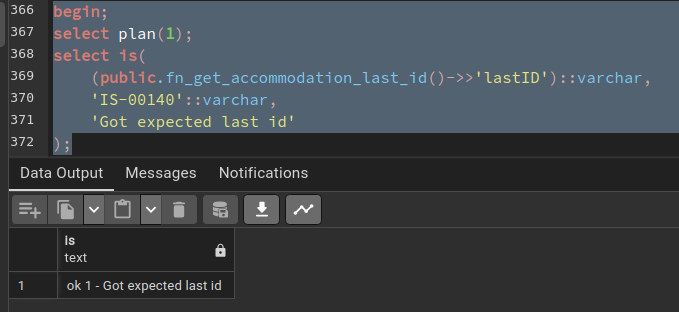
\includegraphics[width=\textwidth]{slike/unit_tests/ut_6/success_invocation.png}
					\caption{Pokretanje testa za provjeru rada same funkcije, uspijeh}
					\label{fig: IS6-uspješno dohvaćen posljednji realestateid}
				\end{figure}
				\begin{figure}[H]
					\centering
					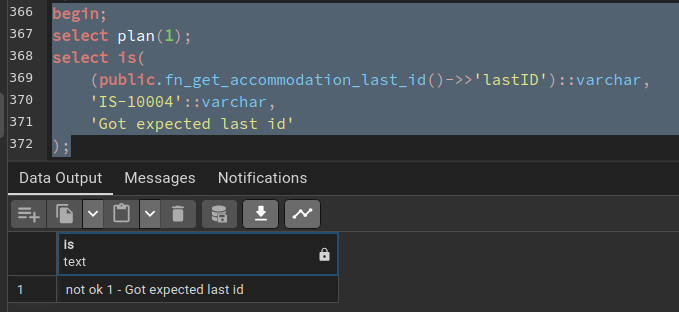
\includegraphics[width=\textwidth]{slike/unit_tests/ut_6/failure_invocation.png}
					\caption{Pokretanje testa za provjeru rada same funkcije, neuspijeh}
					\label{fig: IS6-navedeni realestateid ne postoji}
				\end{figure}
				\begin{figure}[H]
					\centering
					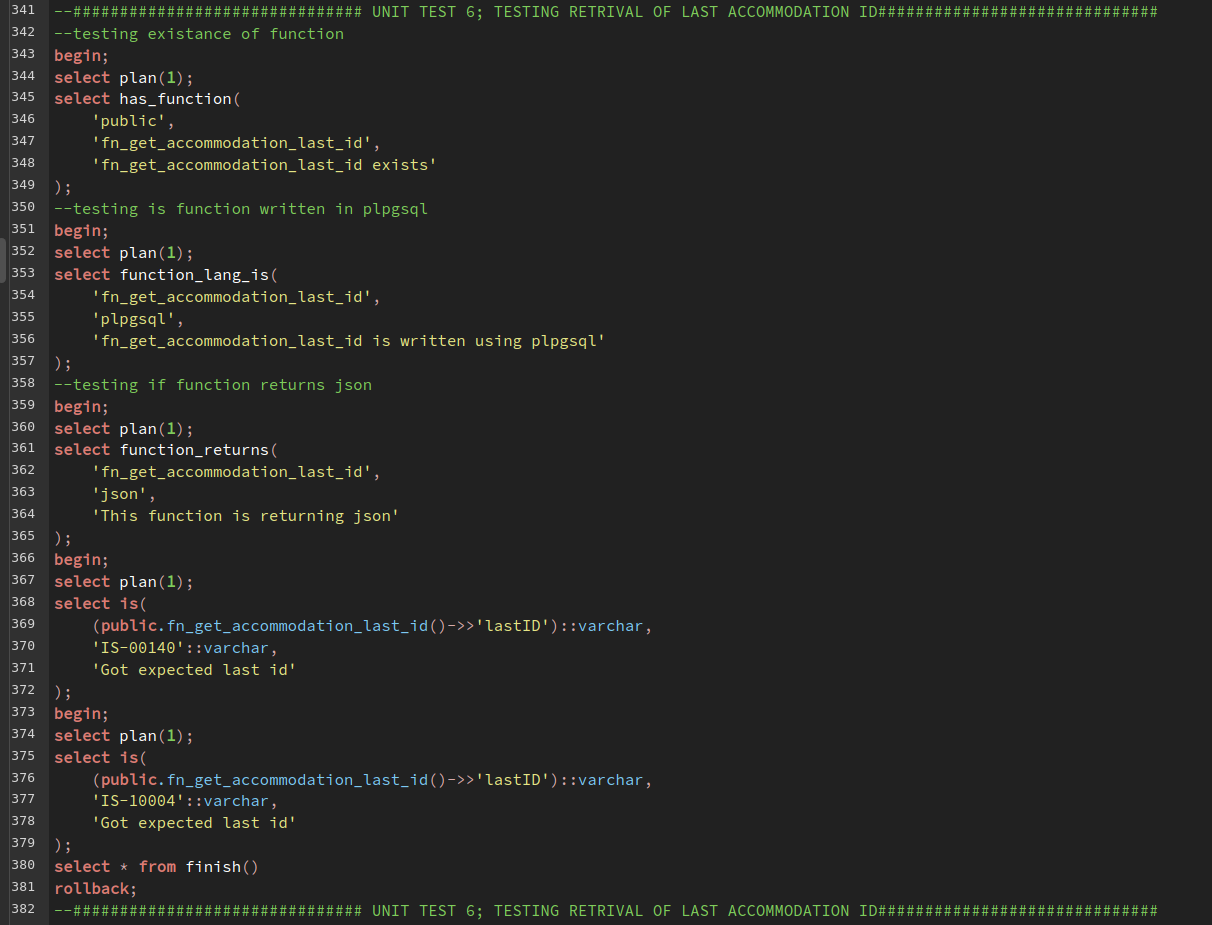
\includegraphics[width=\textwidth]{slike/unit_tests/ut_6/code.png}
					\caption{Kod isptinog slučaja 6}
					\label{fig: IS6-kod}
				\end{figure}
				\eject
			\eject
		\section{Dijagram razmještaja}
			
			\textbf{\textit{dio 2. revizije}}
			
			 \textit{Potrebno je umetnuti \textbf{specifikacijski} dijagram razmještaja i opisati ga. Moguće je umjesto specifikacijskog dijagrama razmještaja umetnuti dijagram razmještaja instanci, pod uvjetom da taj dijagram bolje opisuje neki važniji dio sustava.}
			
			\eject 
		
		\section{Upute za puštanje u pogon}
		
			Aplikacija je puštena u pogon na cloud servisu Render čime smo omogućili javni pristup aplikaciji.
			
			\textbf{\textit{Konfiguracija frontenda}}
			
			\textbf{\textit{Konfiguracija baze/backenda}}
			
			
			\eject 
	\chapter{Zaključak i budući rad}
		
		\textbf{\textit{dio 2. revizije}}\\
		
		 \textit{U ovom poglavlju potrebno je napisati osvrt na vrijeme izrade projektnog zadatka, koji su tehnički izazovi prepoznati, jesu li riješeni ili kako bi mogli biti riješeni, koja su znanja stečena pri izradi projekta, koja bi znanja bila posebno potrebna za brže i kvalitetnije ostvarenje projekta i koje bi bile perspektive za nastavak rada u projektnoj grupi.}
		
		 \textit{Potrebno je točno popisati funkcionalnosti koje nisu implementirane u ostvarenoj aplikaciji.}
		
		\eject 
	\chapter*{Popis literature}
		\addcontentsline{toc}{chapter}{Popis literature}
	 	
 		\textbf{\textit{Kontinuirano osvježavanje}}
	
		\textit{Popisati sve reference i literaturu koja je pomogla pri ostvarivanju projekta.}
		
		
		\begin{enumerate}
			
			
			\item  Programsko inženjerstvo, FER ZEMRIS, \url{http://www.fer.hr/predmet/proinz}
			
			\item  I. Sommerville, "Software engineering", 8th ed, Addison Wesley, 2007.
			
			\item  T.C.Lethbridge, R.Langaniere, "Object-Oriented Software Engineering", 2nd ed. McGraw-Hill, 2005.
			
			\item  I. Marsic, Software engineering book``, Department of Electrical and Computer Engineering, Rutgers University, \url{http://www.ece.rutgers.edu/~marsic/books/SE}
			
			\item  The Unified Modeling Language, \url{https://www.uml-diagrams.org/}
			
			\item  Astah Community, \url{http://astah.net/editions/uml-new}
		\end{enumerate}
		
		 
	
	
	\begingroup
	\renewcommand*\listfigurename{Indeks slika i dijagrama}
	%\renewcommand*\listtablename{Indeks tablica}
	%\let\clearpage\relax
	\listoffigures
	%\vspace{10mm}
	%\listoftables
	\endgroup
	\addcontentsline{toc}{chapter}{Indeks slika i dijagrama}


	
	\eject 
		
	\chapter*{Dodatak: Prikaz aktivnosti grupe}
		\addcontentsline{toc}{chapter}{Dodatak: Prikaz aktivnosti grupe}
		
		\section*{Dnevnik sastajanja}
		
		\begin{packed_enum}
			\item  sastanak
			
			\item[] \begin{packed_item}
				\item Datum:18.10.2023.
				\item Prisustvovali: Karlo Baljak, Luka Kokić, Ian Marković, Mateo Martić, Mislav Matić, Bruno Milaković, Teo Musa
				\item Teme sastanka:
				\begin{packed_item}
					\item  Međusobno upoznavanje
					\item  Rasprava o projektnom zadatku
				\end{packed_item}
			\end{packed_item}
			
			\item  sastanak
			
			\item[] \begin{packed_item}
				\item Datum:25.10.2023.
				\item Prisustvovali: Karlo Baljak, Luka Kokić, Ian Marković, Mateo Martić, Mislav Matić, Bruno Milaković, Teo Musa
				\item Teme sastanka:
				\begin{packed_item}
					\item  Podjela zadataka na projektu
					\item  Rasprava o alatima koje ćemo koristiti
				\end{packed_item}
			\end{packed_item}
			
			\item  sastanak
			
			\item[] \begin{packed_item}
				\item Datum:10.11.2023.
				\item Prisustvovali: Karlo Baljak, Luka Kokić, Ian Marković, Mateo Martić, Mislav Matić, Bruno Milaković, Teo Musa
				\item Teme sastanka:
				\begin{packed_item}
					\item  Rasprava o finalizaciji finijih detalja vezano uz obrasce uporabe i dijagrame te njihova finalizacija
					\item  Raspodjela zadataka koji trebaju biti obavljeni do prve predaje
				\end{packed_item}
			\end{packed_item}
			
			\item  sastanak
			
			\item[] \begin{packed_item}
				\item Datum:6.12.2023.
				\item Prisustvovali: Karlo Baljak, Luka Kokić, Ian Marković, Mateo Martić, Mislav Matić, Bruno Milaković, Teo Musa
				\item Teme sastanka:
				\begin{packed_item}
					\item  Podjela zadataka na projektu u drugom ciklusu
				\end{packed_item}
			\end{packed_item}
			
			\item  sastanak
			
			\item[] \begin{packed_item}
				\item Datum:11.1.2024.
				\item Prisustvovali: Karlo Baljak, Luka Kokić, Ian Marković, Mislav Matić, Bruno Milaković, Teo Musa
				\item Teme sastanka:
				\begin{packed_item}
					\item  Usklađivanje frontend-a i backend-a
					\item  Rasprava o izgledu stranice i o tome kako su podstranice organizirane
					\item  Raspodjela preostalih zadataka
				\end{packed_item}
			\end{packed_item}
			
			%
			
		\end{packed_enum}
		
		\eject
		\section*{Tablica aktivnosti}

			\begin{longtblr}[
					label=none,
				]{
					vlines,hlines,
					width = \textwidth,
					colspec={X[7, l]X[1, c]X[1, c]X[1, c]X[1, c]X[1, c]X[1, c]X[1, c]}, 
					vline{1} = {1}{text=\clap{}},
					hline{1} = {1}{text=\clap{}},
					rowhead = 1,
				} 
			
				\SetCell[c=1]{c}{} & \SetCell[c=1]{c}{\rotatebox{90}{\textbf{Luka Kokić}}} & \SetCell[c=1]{c}{\rotatebox{90}{\textbf{Karlo Baljak}}} &	\SetCell[c=1]{c}{\rotatebox{90}{\textbf{Ian Marković}}} & \SetCell[c=1]{c}{\rotatebox{90}{\textbf{Mateo Martić}}} &	\SetCell[c=1]{c}{\rotatebox{90}{\textbf{Mislav Matić}}} & \SetCell[c=1]{c}{\rotatebox{90}{\textbf{Bruno Milaković}}} &	\SetCell[c=1]{c}{\rotatebox{90}{\textbf{Teo Musa}}} \\  
				Upravljanje projektom 		& 7 &  &  &  &  &  & \\ 
				Opis projektnog zadatka 	&  &  & 4 &  &  &  & \\ 
				
				Funkcionalni zahtjevi       &  &  & 3 &  &  &  &  \\ 
				Opis pojedinih obrazaca 	&  &  & 8 &  &  &  & 8  \\ 
				Dijagram obrazaca 			&  &  &  &  &7  &  &  \\ 
				Sekvencijski dijagrami 		&  &  &  &  &  & 11 &  \\ 
				Opis ostalih zahtjeva 		&  &  & 1 &  &  &  &  \\ 

				Arhitektura i dizajn sustava	 &  & 3 &  &  &  &  &  \\ 
				Baza podataka				&  & 15 &  &  &  &  &   \\ 
				Dijagram razreda 			&  & 5 &  & 5 &  &  &   \\ 
				Dijagram stanja				&  &  &  &  &  &  &  \\ 
				Dijagram aktivnosti 		&  &  &  &  &  &  &  \\ 
				Dijagram komponenti			&  &  &  &  &  &  &  \\ 
				Korištene tehnologije i alati 		&  &  &  &  &  &  &  \\ 
				Ispitivanje programskog rješenja 	&  &  &  &  &  &  &  \\ 
				Dijagram razmještaja			&  &  &  &  &  &  &  \\ 
				Upute za puštanje u pogon 		&  & &  &  &  &  &  \\  
				Dnevnik sastajanja 			& 1 &  &  &  &  &  &  \\ 
				Zaključak i budući rad 		&  &  &  &  &  &  &  \\  
				Popis literature 			&  &  &  &  &1  &  &  \\  
				Ukupno dokumentacija		& 8 & 23 & 16 & 5 & 8 & 11 & 8  \\  
				Sastanci	& 14 & 14 & 14 & 12 & 12 & 12 & 12 \\  
				Istraživanje informacija i tehnologija	& 10 & 13 & 5 & 4 & 4 & 7 & 4\\
				Deployment		&  & 10 &  &  &  &  &  \\  
				Izrada baze podataka	&  & 7 &  &  &  &  & \\  
				Spajanje s bazom podataka	&  & 5 &  &  &  &  &  \\ 
				Backend							& 2 & 10 &  & &  &  &  \\ 
				Frontend				& 3 & 5 &  &  &  &  &  \\
				Ukupno razvoj projekta		& 37 & 87 & 35 & 21 & 24 & 30 & 24 \\   
			\end{longtblr}
					
					
		\eject
		\section*{Dijagrami pregleda promjena}
		
		\textbf{\textit{dio 2. revizije}}\\
		
		\textit{Prenijeti dijagram pregleda promjena nad datotekama projekta. Potrebno je na kraju projekta generirane grafove s gitlaba prenijeti u ovo poglavlje dokumentacije. Dijagrami za vlastiti projekt se mogu preuzeti s gitlab.com stranice, u izborniku Repository, pritiskom na stavku Contributors.}
		
	


\end{document} %naredbe i tekst nakon ove naredbe ne ulaze u izgrađen dokument 


